%% ===================================================================
%%  A Plain-English Guide to the Multi-Scalar PDF Project
%%  Compile with:  tectonic docs/mdn_and_sampling_explained.tex
%%  or:            pixi run doc
%% ===================================================================
\documentclass[11pt,a4paper]{report}

\usepackage[margin=2.4cm]{geometry}
\usepackage{amsmath}
\usepackage{amssymb}
\usepackage{booktabs}
\usepackage{longtable}
\usepackage{array}
\usepackage{xcolor}
\usepackage{enumitem}
\usepackage{microtype}
\usepackage{fancyhdr}
\usepackage{tikz}
\usetikzlibrary{arrows.meta, positioning, shapes.geometric, calc}

\definecolor{NavyBlue}{RGB}{20,60,120}
\definecolor{CodeLink}{RGB}{150,40,40}
\definecolor{TagGray}{RGB}{110,110,110}
\definecolor{BoxBG}{RGB}{244,246,250}
\definecolor{BoxRule}{RGB}{190,200,215}
\definecolor{WarnBG}{RGB}{253,246,236}
\definecolor{WarnRule}{RGB}{220,180,120}

\usepackage[colorlinks=true,linkcolor=NavyBlue,urlcolor=CodeLink,citecolor=NavyBlue]{hyperref}

% -------------------------------------------------------------------
% Source-reference machinery
% -------------------------------------------------------------------
\newcommand{\srcbase}{vscode://file/Users/syellapa/Documents/Research/2026/ANSYS/Multi-ScalarPDF}
\newcommand{\dmdn}{dirichlet\string_mdn}
\newcommand{\srctag}[1]{{\footnotesize\textcolor{TagGray}{[#1]}}}

% Two-argument form: #1 = line number, #2 = display name (escape underscores yourself)
% One-argument "L" form: bare line-number marker, for mid-sentence references.
\newcommand{\Mpi}[2]{\href{\srcbase/EnsightPDFHybridDatasetMPI.py:#1}{\texttt{#2}}\,\srctag{MPI:#1}}
\newcommand{\MpiL}[1]{\href{\srcbase/EnsightPDFHybridDatasetMPI.py:#1}{\srctag{MPI:#1}}}
\newcommand{\Ser}[2]{\href{\srcbase/EnsightPDFHybridDataset.py:#1}{\texttt{#2}}\,\srctag{SER:#1}}

\newcommand{\Model}[2]{\href{\srcbase/\dmdn/model.py:#1}{\texttt{#2}}\,\srctag{MODEL:#1}}
\newcommand{\ModelL}[1]{\href{\srcbase/\dmdn/model.py:#1}{\srctag{MODEL:#1}}}
\newcommand{\Loss}[2]{\href{\srcbase/\dmdn/losses.py:#1}{\texttt{#2}}\,\srctag{LOSS:#1}}
\newcommand{\LossL}[1]{\href{\srcbase/\dmdn/losses.py:#1}{\srctag{LOSS:#1}}}
\newcommand{\Grid}[2]{\href{\srcbase/\dmdn/bin\string_grid.py:#1}{\texttt{#2}}\,\srctag{GRID:#1}}
\newcommand{\Data}[2]{\href{\srcbase/\dmdn/data.py:#1}{\texttt{#2}}\,\srctag{DATA:#1}}
\newcommand{\DataL}[1]{\href{\srcbase/\dmdn/data.py:#1}{\srctag{DATA:#1}}}
\newcommand{\Split}[2]{\href{\srcbase/\dmdn/splits.py:#1}{\texttt{#2}}\,\srctag{SPLIT:#1}}
\newcommand{\Train}[2]{\href{\srcbase/\dmdn/train.py:#1}{\texttt{#2}}\,\srctag{TRAIN:#1}}
\newcommand{\TrainL}[1]{\href{\srcbase/\dmdn/train.py:#1}{\srctag{TRAIN:#1}}}
\newcommand{\Eval}[2]{\href{\srcbase/\dmdn/evaluate.py:#1}{\texttt{#2}}\,\srctag{EVAL:#1}}
\newcommand{\Metric}[2]{\href{\srcbase/\dmdn/metrics.py:#1}{\texttt{#2}}\,\srctag{METRIC:#1}}
\newcommand{\Plot}[2]{\href{\srcbase/\dmdn/plotting.py:#1}{\texttt{#2}}\,\srctag{PLOT:#1}}
\newcommand{\Verify}[2]{\href{\srcbase/\dmdn/verify.py:#1}{\texttt{#2}}\,\srctag{VERIFY:#1}}

\newcommand{\code}[1]{\texttt{#1}}
\newcommand{\term}[1]{\textbf{#1}}

% Long snake_case identifiers are unbreakable by default and cause overfull lines.
% Allow a line break after every underscore in text mode.
\let\origtextunderscore\_
\renewcommand{\_}{\origtextunderscore\allowbreak}
\setlength{\emergencystretch}{3em}

% -------------------------------------------------------------------
% Callout boxes. \colorbox cannot be split across an environment's
% begin/end parts, so the body is captured in a save box first.
% -------------------------------------------------------------------
\newsavebox{\calloutbox}
\newlength{\calloutwidth}
\setlength{\fboxsep}{9pt}

\newcommand{\calloutOpen}{%
  \par\medskip\noindent
  \setlength{\calloutwidth}{\dimexpr\linewidth-2\fboxsep\relax}%
  \begin{lrbox}{\calloutbox}\begin{minipage}{\calloutwidth}}
\newcommand{\calloutClose}[1]{%
  \end{minipage}\end{lrbox}\colorbox{#1}{\usebox{\calloutbox}}\par\medskip}

\newenvironment{plainbox}[1]
  {\calloutOpen\textbf{#1}\par\medskip}
  {\calloutClose{BoxBG}}

\newenvironment{analogy}
  {\calloutOpen\textbf{In everyday terms.}\ }
  {\calloutClose{BoxBG}}

\newenvironment{caution}
  {\calloutOpen\textbf{Watch out.}\ }
  {\calloutClose{WarnBG}}

\pagestyle{fancy}
\fancyhf{}
\fancyhead[L]{\small\nouppercase{\leftmark}}
\fancyhead[R]{\small\thepage}
\renewcommand{\headrulewidth}{0.3pt}

\setlist[itemize]{itemsep=2pt, topsep=4pt}
\setlist[enumerate]{itemsep=3pt, topsep=4pt}

\title{\bfseries How the Multi-Scalar PDF Project Works\\[0.6em]
\large A complete, jargon-free walkthrough of the MPI data-sampling pipeline\\
and the Dirichlet Mixture Density Network}
\author{Generated documentation for the \code{Multi-ScalarPDF} workspace}
\date{\today}

\begin{document}

\maketitle
\thispagestyle{empty}

\vspace{1cm}
\begin{plainbox}{Who this document is for}
You have never worked with turbulent combustion, probability distributions, or neural
networks. You want to understand \emph{exactly} what this code does and why, without
having to look up a single technical term. Every specialised word in this document is
explained the first time it appears, and again in the glossary at the end.
Every time we describe something the code actually does, we tell you the file and the
line number so you can go look at it yourself.
\end{plainbox}

\begin{plainbox}{How to read the source references}
Throughout the text you will see markers like
\Mpi{640}{process\_work\_units\_on\_rank}.
The monospaced part is the name of a function in the code; the grey bracket is a
short file tag plus the line number where that function begins. If you open this PDF
on the machine that holds the code, clicking the name jumps straight to that line in
VS~Code. The file tags are:

\medskip
\begin{tabular}{@{}ll@{}}
\toprule
\textbf{Tag} & \textbf{File} \\
\midrule
\code{MPI}    & \code{EnsightPDFHybridDatasetMPI.py} \\
\code{SER}    & \code{EnsightPDFHybridDataset.py} \\
\code{GRID}   & \code{dirichlet\_mdn/bin\_grid.py} \\
\code{DATA}   & \code{dirichlet\_mdn/data.py} \\
\code{SPLIT}  & \code{dirichlet\_mdn/splits.py} \\
\code{MODEL}  & \code{dirichlet\_mdn/model.py} \\
\code{LOSS}   & \code{dirichlet\_mdn/losses.py} \\
\code{TRAIN}  & \code{dirichlet\_mdn/train.py} \\
\code{EVAL}   & \code{dirichlet\_mdn/evaluate.py} \\
\code{METRIC} & \code{dirichlet\_mdn/metrics.py} \\
\code{PLOT}   & \code{dirichlet\_mdn/plotting.py} \\
\code{VERIFY} & \code{dirichlet\_mdn/verify.py} \\
\bottomrule
\end{tabular}
\end{plainbox}

\newpage
\tableofcontents
\newpage

% ===================================================================
\chapter{The Problem, in Ordinary Language}
% ===================================================================

\section{What is actually being simulated}

Imagine you pour a drop of red dye and a drop of blue dye into a bucket of water and
then stir it violently. At first the two dyes are separate blobs. As you stir, they
stretch into ribbons, then into threads, then into a fine mist of colour, and eventually
they are mixed so thoroughly that every teaspoon of water looks the same shade of purple.

That process --- stirring two substances together in a turbulent fluid --- is what this
project is about. In the real application the two substances are not dyes but two
\term{chemical scalars}: two quantities that get carried around by the flow, such as the
concentration of fuel and the concentration of an additive. We call them \term{scalar~A}
and \term{scalar~B}. At every point in space, at every moment in time, scalar~A has some
value between 0 and 1, and scalar~B has some value between 0 and 1.

There is one extra rule that matters enormously for everything that follows. The two
scalars, plus whatever is left over (the ``background''), must add up to the whole:
\[
  z_1 + z_2 + z_3 = 1, \qquad z_1, z_2, z_3 \ge 0 .
\]
Here $z_1$ is the amount of scalar~A, $z_2$ is the amount of scalar~B, and $z_3 = 1 - z_1 - z_2$
is everything else. Because the three numbers are non-negative and always sum to one, only
\emph{two} of them are free --- once you know $z_1$ and $z_2$, you automatically know $z_3$.

\begin{analogy}
Think of a pie chart with exactly three slices. You can make the slices any size you
like, but they must together fill the whole pie. Once you have chosen the size of the
first two slices, the third is decided for you.
\end{analogy}

\section{The triangle}

If you draw all the possible pairs $(z_1, z_2)$ that obey the rule above, you do not get a
square --- you get a \emph{triangle}. The corners of the triangle are the three ``pure''
states: all scalar~A, all scalar~B, all background. The edges are mixtures of exactly two
ingredients. The middle is a blend of all three.

\begin{center}
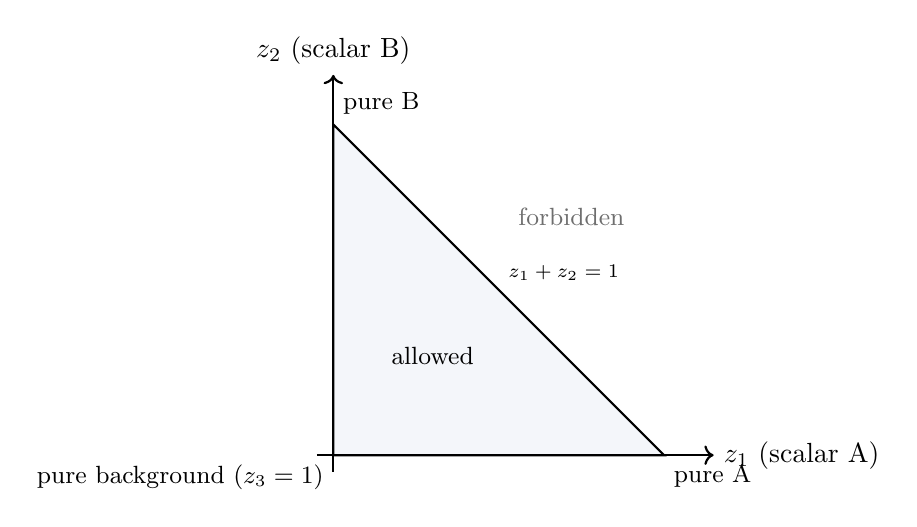
\begin{tikzpicture}[scale=4.2]
  \fill[BoxBG] (0,0) -- (1,0) -- (0,1) -- cycle;
  \draw[thick] (0,0) -- (1,0) -- (0,1) -- cycle;
  \draw[->,thick] (-0.05,0) -- (1.15,0) node[right] {$z_1$ (scalar A)};
  \draw[->,thick] (0,-0.05) -- (0,1.15) node[above] {$z_2$ (scalar B)};
  \node[below left]  at (0,0)   {\small pure background ($z_3=1$)};
  \node[below right] at (1,0)   {\small pure A};
  \node[above right] at (0,1)   {\small pure B};
  \node at (0.3,0.3) {\small allowed};
  \node[TagGray] at (0.72,0.72) {\small forbidden};
  \node at (0.5,0.5) [above right,font=\scriptsize] {$z_1+z_2=1$};
\end{tikzpicture}
\end{center}

\noindent
Mathematicians call this triangle the \term{2-simplex}. You do not need that word, but you
will see it in the code (\code{simplex\_mask}, \code{z\_simplex}, \code{num\_simplex\_cells}),
so it is worth knowing that ``simplex'' simply means ``the triangle of allowed values''.
The upper-right half of the square, where $z_1 + z_2 > 1$, is physically impossible: it
would mean the two ingredients together add up to more than the whole. A rectangular
histogram cell can straddle the diagonal boundary: part of it is allowed and part is not.
The code therefore clips every rectangle against the triangle.  The boolean array
\code{simplex\_mask} is true whenever the clipped piece has positive area.  It does
\emph{not} merely test the rectangle's centre.  This distinction prevents valid
boundary-adjacent cells from disappearing.

\section{Two levels of detail: fine and coarse}

The reference data for this project comes from a \term{Direct Numerical Simulation}, or
\term{DNS}. That is a brute-force computer simulation of the fluid that resolves every
swirl, down to the smallest one that physically exists. In this project each DNS snapshot
is a cube of $256 \times 256 \times 256$ grid cells --- about 16.8 million little boxes,
each holding one value of scalar~A and one value of scalar~B.

DNS is extraordinarily expensive. Engineers who design real burners cannot afford it. They
run a cheaper simulation called \term{LES} (Large Eddy Simulation), which uses far coarser
cells --- say $64 \times 64 \times 64$ DNS cells lumped into a single LES cell. An LES cell
knows only \emph{averages}: it knows the average amount of scalar~A inside it, and how much
that amount wobbles, but it has thrown away the fine-grained detail of what is going on
inside.

That lost detail matters, because chemistry is nonlinear: the average of a reaction rate
is not the reaction rate of the average. To recover the chemistry you need to know the full
\term{distribution} of values inside the cell, not just the average.

\begin{analogy}
Knowing that the average household income in a city is \$60{,}000 tells you very little.
A city where everyone earns exactly \$60{,}000 behaves completely differently from a city
where half the people earn \$10{,}000 and half earn \$110{,}000. The \emph{spread and shape}
of the values is the missing information.
\end{analogy}

\section{The central question of the whole project}

\begin{plainbox}{The one sentence that explains everything}
Given only a handful of summary numbers about an LES cell (the averages and the wobble),
can we reconstruct the full distribution of scalar values inside that cell?
\end{plainbox}

The project answers that question in two halves:

\begin{enumerate}
  \item \textbf{The sampling pipeline} (Chapters~\ref{ch:sampling-overview}--\ref{ch:outputs})
        chops DNS cubes into millions of virtual LES cells, computes both the summary numbers
        \emph{and} the true distribution for each, throws away redundant examples, and stores
        the survivors on disk. This is the ``textbook'' the neural network will study.
  \item \textbf{The Dirichlet Mixture Density Network}
        (Chapters~\ref{ch:mdn-idea}--\ref{ch:eval}) is a small neural network that reads the
        summary numbers and outputs a compact mathematical description of the full distribution.
\end{enumerate}

\section{What a ``distribution'' looks like here}

Take one LES-sized cube of DNS data, say $64^3 = 262{,}144$ fine cells. Each of those fine
cells gives you one pair $(z_1, z_2)$ --- one dot inside the triangle. Plot all 262{,}144 dots
and you get a cloud. Some regions of the triangle are crowded; some are empty.

To store that cloud compactly we lay a grid of small squares over the triangle and simply
count how many dots land in each square, then divide by the total. The result is a table of
$64 \times 64 = 4096$ numbers that add up to exactly 1. This table is called a
\term{histogram}, or in this project a \term{joint PDF} (``PDF'' = probability density function;
``joint'' = of two variables at once).

\begin{plainbox}{Vocabulary you now own}
\begin{itemize}
  \item \term{Scalar}: a quantity carried by the flow, valued between 0 and 1.
  \item \term{Simplex / triangle}: the set of allowed $(z_1, z_2)$ pairs.
  \item \term{DNS}: the fine, expensive, reference simulation.
  \item \term{LES cell / filter box}: a cube of many DNS cells, treated as one coarse cell.
  \item \term{Histogram / joint PDF}: a $64\times64$ table of fractions summing to 1, describing
        how the values inside one filter box are spread over the triangle.
  \item \term{Moments}: the summary numbers (averages and wobble) --- defined properly in
        Section~\ref{sec:moments}.
\end{itemize}
\end{plainbox}

% ===================================================================
\chapter{The Sampling Pipeline: Bird's-Eye View}
\label{ch:sampling-overview}
% ===================================================================

The sampling program is \code{EnsightPDFHybridDatasetMPI.py}. Its job is to turn raw
simulation output into a curated training set. The word \term{MPI} in the filename means the
program can run on many CPU cores --- even many separate computers --- at the same time.
We will unpack that in Chapter~\ref{ch:mpi}.

This is the canonical implementation. The shorter
\code{EnsightPDFHybridDataset.py} imports and calls it with one MPI rank, so serial and
parallel runs cannot quietly drift into two different algorithms.

\section{The nine stages}

\begin{center}
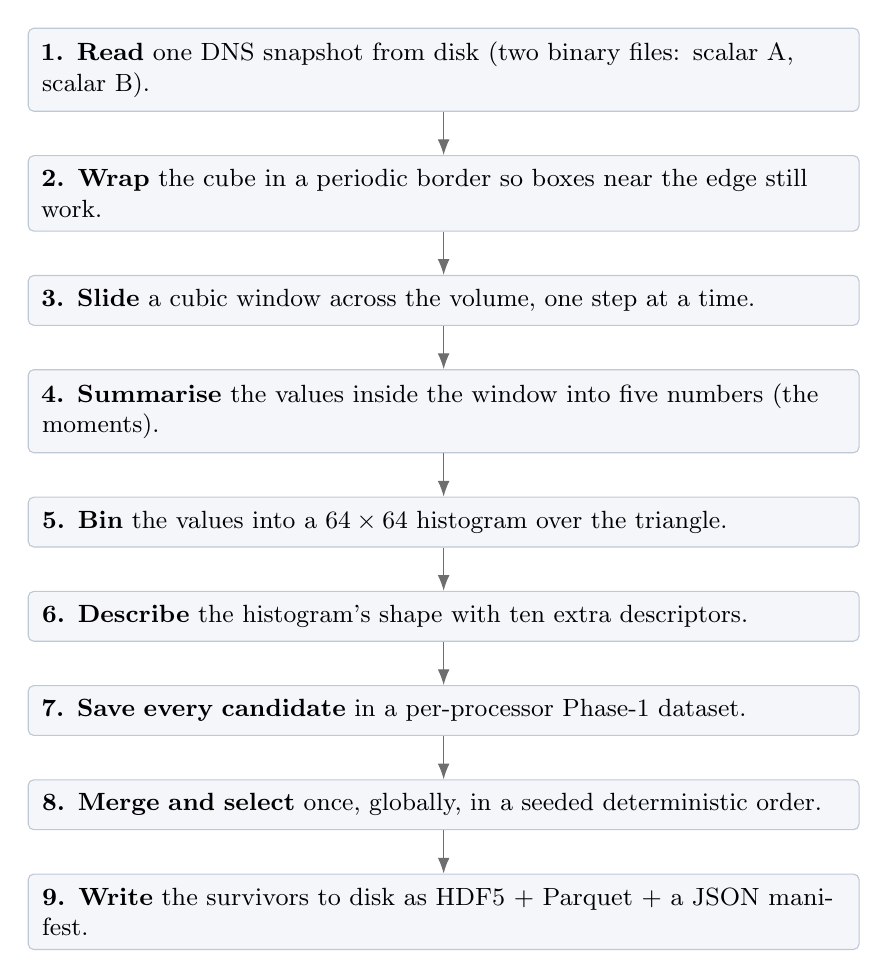
\begin{tikzpicture}[
  node distance=5.5mm,
  every node/.style={font=\small},
  box/.style={draw=BoxRule, fill=BoxBG, rounded corners=2pt,
              text width=10.2cm, align=left, inner sep=5pt},
  arrow/.style={-{Latex[length=2mm]}, draw=TagGray}
]
\node[box] (a) {\textbf{1. Read} one DNS snapshot from disk (two binary files: scalar A, scalar B).};
\node[box, below=of a] (b) {\textbf{2. Wrap} the cube in a periodic border so boxes near the edge still work.};
\node[box, below=of b] (c) {\textbf{3. Slide} a cubic window across the volume, one step at a time.};
\node[box, below=of c] (d) {\textbf{4. Summarise} the values inside the window into five numbers (the moments).};
\node[box, below=of d] (e) {\textbf{5. Bin} the values into a $64\times64$ histogram over the triangle.};
\node[box, below=of e] (f) {\textbf{6. Describe} the histogram's shape with ten extra descriptors.};
\node[box, below=of f] (g) {\textbf{7. Save every candidate} in a per-processor Phase-1 dataset.};
\node[box, below=of g] (h) {\textbf{8. Merge and select} once, globally, in a seeded deterministic order.};
\node[box, below=of h] (i) {\textbf{9. Write} the survivors to disk as HDF5 + Parquet + a JSON manifest.};
\draw[arrow] (a) -- (b);
\draw[arrow] (b) -- (c);
\draw[arrow] (c) -- (d);
\draw[arrow] (d) -- (e);
\draw[arrow] (e) -- (f);
\draw[arrow] (f) -- (g);
\draw[arrow] (g) -- (h);
\draw[arrow] (h) -- (i);
\end{tikzpicture}
\end{center}

Stages 1--7 happen inside \Mpi{640}{process\_work\_units\_on\_rank}; stage 8 is
\Mpi{881}{merge\_per\_rank\_outputs}; stage 9 is \Mpi{533}{materialize\_dataset}. The
conductor that calls all of them in order is \Mpi{1047}{main}.

\section{The scale of the thing}

To make the numbers concrete, here is what the real production run actually did, taken
straight from the manifest file it wrote
(\code{hybrid\_dataset\_mpi/all\_cases\_w64\_w128\_manifest.json}):

\begin{center}
\begin{tabular}{@{}lr@{}}
\toprule
\textbf{Quantity} & \textbf{Value} \\
\midrule
Distinct simulation runs                      & 27 \\
Distinct scalar configurations                & 8 \\
Timesteps per run                             & 13 \\
Filter box sizes                              & $64^3$ and $128^3$ \\
Histogram resolution                          & $64 \times 64$ \\
Windows examined in Phase 1                   & 2{,}156{,}544 \\
Candidates surviving Phase 1 into the merge   & 825{,}249 \\
Examples finally retained                     & 165{,}895 \\
Output HDF5 shard files                        & 7 \\
Wall-clock time of the merge                  & about 3 hours \\
\bottomrule
\end{tabular}
\end{center}

So roughly \emph{one in thirteen} of the windows examined survived to the final dataset.
Chapter~\ref{ch:retention} explains precisely how that filtering decision is made, because
it is the most interesting and least obvious part of the pipeline.

% ===================================================================
\chapter{Stage 1--2: Reading and Padding the Simulation Data}
% ===================================================================

\section{How the data is laid out on disk}

The DNS output lives in a directory tree that looks like this:

\begin{center}
\begin{tabular}{@{}l@{}}
\toprule
\code{<root>/run\_0000/ensight-3D/ZAI1\_0/ZAI1\_0.000017} \\
\code{<root>/run\_0000/ensight-3D/ZBI1\_0/ZBI1\_0.000017} \\
\code{<root>/run\_0001/ensight-3D/...} \\
\bottomrule
\end{tabular}
\end{center}

Reading left to right: \code{run\_0000} is one simulation; \code{ZA} and \code{ZB} mark
scalar~A and scalar~B; \code{I1} is the \term{scalar configuration} (a label for which
initial arrangement of the two dyes was used --- the eight labels are listed at
\MpiL{41}: \code{I1, I4, I5, L1, PI1, PI4, PI5, PL1}); and \code{000017} is the timestep
number. The path construction happens inside
\Mpi{640}{process\_work\_units\_on\_rank}, which first checks that the run folder exists,
then the \code{ensight-3D} folder, then the two scalar folders, then the individual
timestep files --- recording a friendly message in a \code{missing\_paths} list for each
thing it cannot find, and only crashing if you passed \code{--strict-missing}.

\begin{caution}
Missing files are \emph{not} fatal by default. This is deliberate: a 27-run sweep with a
few incomplete runs should still produce a usable dataset. But it means you should always
read the \code{missing\_paths} section of the output manifest before trusting a dataset.
\end{caution}

\section{Undoing the parallel decomposition}

\Mpi{104}{read\_ensight} does the actual file reading, and it has to undo something the
original simulation did.

The DNS was itself computed in parallel, on $8 \times 8 \times 8 = 512$ processors. Each
processor owned a small sub-cube of $32^3$ cells and wrote its own piece. The file on disk
is therefore not a simple ``row by row'' dump of the big cube; it is 512 small cubes
stacked one after another.

The reading procedure is:

\begin{enumerate}
  \item Skip four header blocks --- three 80-byte text banners and one 4-byte integer
        (\MpiL{107}). These hold descriptive text the code does not need.
  \item Read the rest of the file as one long list of 4-byte floating-point numbers.
  \item Reshape that list into a six-dimensional array with shape
        $(32, 32, 32, 8, 8, 8)$: the first three indices say ``where inside a sub-cube'',
        the last three say ``which sub-cube''. The \code{order="F"} flag tells the reshape
        to fill the first index fastest, matching how Fortran (which wrote the file) stores
        arrays.
  \item Loop over the 512 sub-cubes and copy each into its correct slot in a fresh
        $256^3$ array. Note the index order \code{[:, :, :, kp, jp, ip]} --- the processor
        indices are read back-to-front, which is exactly the transposition needed to undo
        the Fortran ordering.
\end{enumerate}

The same procedure runs twice, once for scalar~A and once for scalar~B, and the function
returns the two padded cubes.

\begin{caution}
The constants $256$ (\code{--nx}) and $8$ (\code{--npx}) are command-line options, defaulting
to the values above. If you point this script at a simulation with a different resolution or
a different processor layout and forget to change them, the reshape will either crash or,
worse, silently scramble the data. There is no header check that catches this.
\end{caution}

\section{Wrapping the cube: periodic padding}
\label{sec:padding}

Now a practical problem. We want to slide a $64^3$ window over the cube. What happens when
the window's centre is near a face of the cube? Half the window would hang off the edge.

The physics gives us the answer for free. These simulations are \term{periodic}: the cube is
a tile in an infinite, repeating pattern. Whatever leaves through the right face re-enters
through the left. So we can simply glue copies of the opposite faces onto each side.

\Mpi{87}{fill\_periodic} does this. It creates a bigger array of size
$(256 + 2w)^3$ where $w$ is the padding width, drops the original cube into the middle, and
then fills the borders:

\begin{itemize}
  \item Lines \MpiL{92}--\MpiL{93} fill the two ends of the first axis by copying the last
        $w$ slices to the front and the first $w$ slices to the back.
  \item Lines \MpiL{95}--\MpiL{96} then do the second axis --- but note they operate on
        \code{mod}, the already-partially-filled array, not on \code{orig}. That is what makes
        the corners come out right without extra code.
  \item Lines \MpiL{98}--\MpiL{99} do the same for the third axis.
\end{itemize}

The padding width is chosen once in \Mpi{1047}{main} at \MpiL{1088} as
\code{pad\_width = max(width // 2 for width in box\_widths)} --- half of the largest filter box.
With boxes of 64 and 128 that gives $w = 64$, so the padded array is $384^3$. In memory that
is about 226~MB per scalar as 32-bit floats, or roughly 450~MB for the pair. This is the
single largest memory consumer per processor during Phase~1.

\begin{analogy}
Periodic padding is like the wrap-around in old arcade games: fly off the right edge of the
screen and you reappear on the left. Padding just pre-draws that wrap-around so the sliding
window never has to think about edges.
\end{analogy}

% ===================================================================
\chapter{Stage 3: The Sliding Window}
% ===================================================================

\section{What the window is and how it moves}

\Mpi{414}{iter\_filter\_records} is the generator that walks the volume. In Python, a
\emph{generator} is a function that hands back results one at a time instead of building a
giant list --- essential here, because building a list of two million histograms would need
terabytes of memory.

The geometry, from \MpiL{415} onward:

\begin{itemize}
  \item \code{half\_width = box\_width // 2}. The command-line option \code{--box-widths}
        gives the \emph{full} cube edge (e.g. 64), and the code halves it internally.
  \item Three identical loops run over centre positions
        \code{range(pad\_width, nx + pad\_width, stride)}: they start at the beginning of the
        real data inside the padded array, run to its end, and step by \code{stride}.
  \item For each centre $(i, j, k)$ the window is the slice
        $[i-h : i+h]$ in each direction --- exactly \code{box\_width} cells on a side.
\end{itemize}

With \code{nx = 256} and \code{stride = 32}, each axis yields $256/32 = 8$ positions, so
$8^3 = 512$ windows per snapshot for the $64^3$ boxes. With \code{stride = 64} for the
$128^3$ boxes you get $4^3 = 64$ windows. Multiply by 27 runs $\times$ 8 configurations
$\times$ 13 timesteps and you land near the 2.16 million figure in the manifest.

\begin{plainbox}{Stride versus box width}
\code{stride} is how far the window jumps between samples; \code{box\_width} is how big the
window is. Because the stride (32) is smaller than the box (64), consecutive windows
\emph{overlap} by half. Overlapping is intentional --- it produces more training examples and
smoother coverage --- but it also means neighbouring examples are correlated, which is one
reason the redundancy filter in Chapter~\ref{ch:retention} exists.
\end{plainbox}

\section{What comes out of each window}

For every window the generator flattens the two sub-cubes into two long lists of numbers
(\code{z1\_values} and \code{z2\_values}, converted to 64-bit precision so the sums stay
accurate), then produces:

\begin{enumerate}
  \item five \term{moments} computed directly from the raw values,
  \item a $64\times64$ histogram,
  \item the same five moments recomputed \emph{from} the histogram, as a cross-check,
  \item ten shape descriptors,
  \item bookkeeping: which run, which configuration, which timestep, which box width,
        which stride, the window centre, and the number of DNS cells inside.
\end{enumerate}

All of that is packed into a Python dictionary \MpiL{434} and yielded together with the
histogram as a pair. One important detail: the centre coordinates recorded in the metadata
have \code{pad\_width} subtracted off, so they refer to the \emph{original} cube, not the
padded one --- see the three \code{center\_i/j/k} entries.

% ===================================================================
\chapter{Stage 4: The Five Summary Numbers (Moments)}
\label{sec:moments}
% ===================================================================

\section{What each number means}

\Mpi{215}{compute\_direct\_moments} produces five numbers from the raw values inside one
window. In plain language:

\begin{center}
\begin{tabular}{@{}llp{8.6cm}@{}}
\toprule
\textbf{Name} & \textbf{Symbol} & \textbf{What it tells you} \\
\midrule
\code{mean\_a} & $\overline{z_1}$ & The average amount of scalar~A in the box. \\[2pt]
\code{var\_a}  & $\widetilde{z_1'^2}$ & How much the amount of A wobbles from cell to cell.
                Zero means perfectly uniform; large means very patchy. \\[2pt]
\code{mean\_b} & $\overline{z_2}$ & The average amount of scalar~B. \\[2pt]
\code{var\_b}  & $\widetilde{z_2'^2}$ & The wobble of scalar~B. \\[2pt]
\code{cov\_ab} & $\widetilde{z_1'z_2'}$ & Whether A and B wobble \emph{together}. Positive:
                where there is a lot of A there tends to be a lot of B. Negative: they avoid
                each other. Zero: no relationship. \\
\bottomrule
\end{tabular}
\end{center}

The formulas, exactly as coded:
\begin{align}
  \overline{z_1} &= \frac{1}{N}\sum_{n=1}^{N} z_1^{(n)}, &
  \widetilde{z_1'^2} &= \frac{1}{N}\sum_{n=1}^{N}\left(z_1^{(n)} - \overline{z_1}\right)^2, \\[4pt]
  \overline{z_2} &= \frac{1}{N}\sum_{n=1}^{N} z_2^{(n)}, &
  \widetilde{z_2'^2} &= \frac{1}{N}\sum_{n=1}^{N}\left(z_2^{(n)} - \overline{z_2}\right)^2, \\[4pt]
  \widetilde{z_1'z_2'} &= \frac{1}{N}\sum_{n=1}^{N}\left(z_1^{(n)} - \overline{z_1}\right)
                                                  \left(z_2^{(n)} - \overline{z_2}\right).
                                                  & &
\end{align}
Here $N$ is the number of DNS cells in the window ($64^3$ or $128^3$).

\begin{analogy}
The mean is the centre of gravity of the dot cloud in the triangle. The two variances say
how far the cloud spreads left--right and up--down. The covariance says whether the cloud is
tilted like a diagonal cigar, and which way it leans.
\end{analogy}

\begin{caution}
The divisor is $N$, not $N-1$. Statisticians call this the \emph{biased} or \emph{population}
variance. It is the right choice here because the window \emph{is} the whole population we
care about, not a sample drawn from a larger one. But if you ever compare these numbers to
values produced by another tool, check which convention that tool uses.
\end{caution}

\section{The same numbers, computed a second way}

\Mpi{237}{compute\_histogram\_moments} recomputes all five moments, but from the histogram
instead of from the raw values. Because the histogram has already thrown away the exact
positions of the dots inside each little square, the two answers will differ slightly. The
size of that difference is a direct measurement of how much resolution the histogram lost.

The code stores both sets --- \code{mean\_a} and \code{hist\_mean\_a}, and so on --- plus a
single worst-case number, \code{moment\_abs\_err\_max}, which is the largest absolute
difference across all five \MpiL{451}. If you ever suspect the binning is too coarse, sort
the metadata by that column and look at the worst offenders.

\begin{caution}
The neural network is trained on the \emph{direct} moments (the raw-value ones), not the
histogram ones. This is a deliberate choice: at deployment time an LES solver would supply
true moments, not histogram-derived ones. The histogram moments measure information lost by
binning. Their maximum disagreement is also an input-quality gate: training stops if it exceeds
the configured tolerance.
\end{caution}

\begin{plainbox}{Reading the variance-regime diagnostic correctly}
For a scalar between 0 and 1 with mean $m$, the largest possible variance is $m(1-m)$.
The diagnostic plots the ratio $\mathrm{variance}/[m(1-m)]$. A ratio near zero means values
are clustered near their mean: the well-mixed limit. A ratio near one means values are split
toward extremes: a highly segregated limit. Earlier labels reversed these meanings; the code
now reports \code{well\_mixed\_lt\_0\_1} and
\code{highly\_segregated\_gt\_0\_8}.
\end{plainbox}

% ===================================================================
\chapter{Stage 5: Building the Histogram}
% ===================================================================

\section{Why the bins are not evenly spaced}

The obvious way to divide the interval from 0 to 1 into 64 bins is to make them all the same
width, $1/64$ each. The code does \emph{not} do that by default, and the reason is physical.

In combustion there is a special mixture ratio, the \term{stoichiometric} value, at which
fuel and oxidiser are present in exactly the proportions the chemical reaction wants. The
flame lives there. In these simulations that special value is small --- the default is
$z_{\text{st}} = 0.1$. Almost all the interesting physics is squeezed into the bottom tenth of
the range, and evenly spaced bins would waste most of their resolution on the boring upper
region.

So the code uses \emph{fine} bins below $z_{\text{st}}$ and \emph{progressively coarser} bins
above it.

\section{Exactly how the bin centres are placed}

\Mpi{149}{get\_bin\_centers} builds the 64 bin centres in two pieces. Let $N = 64$ be the
number of bins and let $c = N/2 = 32$ be the cut index.

\paragraph{Lower half: evenly spaced.}
The first 32 centres march linearly from 0 up to $z_{\text{st}}$:
\[
  \Delta z = \frac{z_{\text{st}}}{c-1}, \qquad
  z_i = i\,\Delta z \quad \text{for } i = 0, 1, \dots, c-1 .
\]
With $z_{\text{st}} = 0.1$ and $c = 32$ that is $\Delta z \approx 0.00323$ --- bins about
twenty times finer than uniform binning would give.

\paragraph{Upper half: a quadratic that speeds up.}
For $i \ge c$ the centres follow a parabola,
\[
  z_i = a\,i^2 + b\,i + \gamma ,
\]
whose three coefficients are pinned down by three requirements:
\begin{enumerate}
  \item the last bin centre must land exactly on 1: \quad $z_{N-1} = 1$;
  \item the curve must pass through $z_{\text{st}}$ at the joint: \quad $z_{c-1} = z_{\text{st}}$;
  \item the spacing must be continuous at the joint, i.e.\ the derivative there equals
        $\Delta z$, so there is no sudden jump in bin width.
\end{enumerate}
Conditions 1 and 3 give a $2\times2$ linear system, solved explicitly in the code by Cramer's
rule (the variables \code{m11}, \code{m12}, \code{m21}, \code{m22}, \code{r1}, \code{r2},
\code{delta}); condition 2 then fixes the constant term \code{coef\_c}. The result is a bin
layout that starts fine, widens smoothly, and reaches 1 exactly at the last bin.

If you pass \code{--uniform-bins}, the whole construction is skipped and
\code{np.linspace(0, 1, num\_bins)} is used instead.

\section{From centres to edges to areas}

\Mpi{177}{get\_histogram\_layout} takes the centres and produces everything else:

\begin{itemize}
  \item \textbf{Edges.} Interior edges sit halfway between neighbouring centres,
        $e_i = \tfrac{1}{2}(z_i + z_{i-1})$. The two outermost edges are extrapolated by
        reflecting the first and last half-gaps. There are $N+1 = 65$ edges for $N = 64$ bins.
  \item \textbf{Clipped cell areas.} Each rectangle is cut at $z_1=0$, $z_2=0$, and
        $z_1+z_2=1$.  \code{cell\_area} stores the area of the surviving polygon, not the
        whole rectangle.  All stored areas add to $1/2$, the exact area of the unit triangle.
        Areas matter when converting a cell's probability into probability per unit area.
  \item \textbf{Clipped centroids.} \code{cell\_centroid\_a} and
        \code{cell\_centroid\_b} store the balance point of each surviving polygon.  The
        likelihood evaluates density there.  A boundary cell's centroid is inside the
        triangle even when its original rectangular centre was outside.
  \item \textbf{Simplex mask.} This is true precisely where clipped area is positive.
\end{itemize}

Of the 4096 cells in the grid, only about 2200 fall inside the triangle. Everything
downstream --- the neural network's loss, the error metrics, the plots --- works only on those
in-triangle cells.

\section{Counting the dots}

\Mpi{224}{compute\_histogram\_pdf} is deceptively short:

\begin{enumerate}
  \item \code{np.histogram2d} counts how many $(z_1, z_2)$ pairs fall into each rectangle,
        using the edge arrays computed above. \code{density=False} means give raw counts.
  \item If the total count is zero the function raises an error --- a guard against
        empty or corrupted windows.
  \item Verify that the histogram counted every validated pair.  A mismatch is an error,
        rather than silently dropping samples outside the bin edges.
  \item Divide by the total. The result is a table of fractions that sums to
        exactly 1.
\end{enumerate}

Before counting, \code{prepare\_scalar\_samples} checks that both scalar arrays have the
same size, every number is finite, each scalar lies in $[0,1]$, and the pair obeys
$z_1+z_2\leq1$. Tiny round-off errors within \code{--scalar-tolerance} are clipped or
projected back to the boundary. Larger errors either stop the run (the default) or are
explicitly dropped by \code{--invalid-scalar-policy drop}. Raw, invalid, adjusted, and
used pair counts are written to the manifest, so this cleaning cannot be hidden.

\begin{caution}
The stored quantity is a \emph{probability mass} per cell, not a probability \emph{density}.
The distinction is: mass = density $\times$ area. Because the cell areas here vary by a
factor of tens across the grid, confusing the two produces badly wrong pictures. The
training code is careful about this: see the \code{log\_cell\_area} buffer in
\Loss{80}{HistogramNLL}, discussed in Section~\ref{sec:nll}.
\end{caution}

The histogram is converted to 32-bit floats before being yielded, halving its memory
footprint. At $64\times64$ that is 16~kB per example. The corrected Phase~1 is lossless
and keeps only one output shard in memory. When the shard reaches
\code{--hdf5-shard-size} records, it is written and the in-memory lists are cleared.
The default bound is 25{,}000 histograms per processor; lowering it reduces memory and
creates more files.

% ===================================================================
\chapter{Stage 6: Describing the Shape of a Histogram}
% ===================================================================

Two histograms can have identical means and variances and still look completely different ---
one a single blob in the middle, the other two blobs at opposite corners. To detect this the
code computes ten \term{shape features}, listed by name at \MpiL{43}.

\section{The three global descriptors}

\Mpi{264}{compute\_shape\_features} first flattens the histogram and computes:

\paragraph{Normalised entropy (\code{shape\_entropy}).}
\[
  H = \frac{-\sum_{m} p_m \log p_m}{\log M}, \qquad M = 4096 .
\]
Entropy measures spread-out-ness. It is 0 when all the probability sits in one cell and 1
when it is spread perfectly evenly over all cells. Dividing by $\log M$ makes the answer sit
between 0 and 1 regardless of grid size. The code clips values at $10^{-16}$ before taking
the logarithm \MpiL{266} so that empty cells do not produce $\log 0 = -\infty$.

\paragraph{Peak height (\code{shape\_max\_prob}).}
Simply the largest single value in the table. A tall peak means the mixture is nearly uniform
inside the box; a low peak means the values are scattered.

\paragraph{Effective support (\code{shape\_effective\_support}).}
\[
  S = \frac{1}{M}\cdot\frac{1}{\sum_m p_m^2} .
\]
The quantity $1/\sum p_m^2$ is the ``effective number of occupied cells''. If probability is
spread evenly over exactly $n$ cells, it evaluates to exactly $n$. Dividing by $M$ turns it
into a fraction of the grid.

\begin{analogy}
Entropy and effective support both answer ``how spread out is this?'' but they weight the
tails differently. Entropy notices faint, wide tails; effective support mostly ignores them
and reports where the bulk of the mass is.
\end{analogy}

\section{The seven regional descriptors}

\Mpi{246}{build\_shape\_masks} pre-computes seven boolean stencils over the triangle --- once,
at program start, not per window --- and \code{compute\_shape\_features} just sums the
probability underneath each:

\begin{center}
\begin{tabular}{@{}lp{9.4cm}@{}}
\toprule
\textbf{Feature} & \textbf{Region it measures} \\
\midrule
\code{shape\_corner\_z1} & Near the ``pure A'' corner: $z_1 \ge 1 - \tau_c$ and $z_2 \le \tau_c$. \\
\code{shape\_corner\_z2} & Near the ``pure B'' corner. \\
\code{shape\_corner\_z3} & Near the ``pure background'' corner: both $z_1$ and $z_2$ small. \\
\code{shape\_edge\_z1\_zero} & Along the edge where A is absent: $z_1 \le \tau_e$. \\
\code{shape\_edge\_z2\_zero} & Along the edge where B is absent. \\
\code{shape\_edge\_z3\_zero} & Along the hypotenuse where the background is absent, i.e.\
                              $1 - z_1 - z_2 \le \tau_e$. \\
\code{shape\_center\_mass}   & Within radius $r$ of the triangle's balance point
                              $(\tfrac13, \tfrac13)$. \\
\bottomrule
\end{tabular}
\end{center}

The three thresholds are command-line options: $\tau_c$ is \code{--corner-threshold}
(default 0.08), $\tau_e$ is \code{--edge-threshold} (default 0.04), and $r$ is
\code{--center-radius} (default 0.12). Every mask is intersected with the triangle mask, so
no region ever extends into forbidden territory.

Physically, corner mass means unmixed pockets survive; centre mass means the box is
well-blended; edge mass means one ingredient is locally missing.

\begin{caution}
These ten features are recorded in the output metadata and are useful for slicing and
plotting the dataset. They are \emph{not} used to make the keep-or-discard decision --- that
uses a different measure entirely, described next.
\end{caution}

% ===================================================================
\chapter{Stage 7: Deciding What to Keep}
\label{ch:retention}
% ===================================================================

This is the heart of the sampler, and the part most worth understanding.

\section{The problem: two million near-identical examples}

The sliding window overlaps itself, adjacent timesteps look alike, and most of the volume at
most times is simply ``well-mixed, nothing interesting''. A naive dataset would be 90\%
redundant, which wastes disk, wastes training time, and --- most damagingly --- teaches the
network that boring cases are what matter.

The solution has two layers: first spread examples evenly across the space of possible
moments, then within each region keep only genuinely different-looking histograms.

\section{Layer 1: chopping moment space into pigeonholes}

\Mpi{349}{compute\_moment\_bin} converts the five moments into five small integers, which
together form a \term{bin key}. The recipe per moment:

\begin{enumerate}
  \item Look up the allowed range \MpiL{350}:
        means run $[0, 1]$; variances run $[0, V]$ where $V$ is \code{--variance-limit}
        (default 0.25); covariance runs $[-C, +C]$ where $C$ is \code{--covariance-limit}
        (default 0.25).
  \item Clamp the value into that range. The clamp uses \code{np.nextafter(high, low)} rather
        than \code{high} itself, so a value sitting exactly at the top does not round up into
        a non-existent bin.
  \item Rescale to $[0, 1)$ and multiply by the number of bins for that moment
        (\code{--moment-bins}, default \code{12,12,12,12,12}).
  \item Truncate to an integer and clamp again for safety.
\end{enumerate}

With twelve divisions per moment there are $12^5 = 248{,}832$ conceivable pigeonholes, though
only a small fraction ever get used, because real moments are strongly correlated --- a box
with mean A near 1 cannot also have a large variance.

Each pigeonhole is allowed to hold at most \code{--max-per-moment-bin} examples (default 50).
That single cap is what makes the final dataset balanced: a rare, extreme moment combination
gets the same 50 slots as the most common one.

\begin{analogy}
Imagine sorting photographs into a chest of drawers labelled by subject, and refusing to put
more than 50 photos in any one drawer. Even if you took 10{,}000 pictures of your cat, only
50 make the album --- so the album ends up showing your whole life, not just your cat.
\end{analogy}

\section{Layer 2: measuring how different two histograms are}

Within a drawer we still need to choose \emph{which} 50 to keep. The criterion is visual
distinctness, measured by the \term{Jensen--Shannon distance}, implemented in
\Mpi{286}{jensen\_shannon\_distance}.

The idea in three steps. Given two histograms $p$ and $q$:
\begin{enumerate}
  \item Form their average, $m = \tfrac{1}{2}(p + q)$.
  \item Ask how surprised you would be by $p$ if you expected $m$, and vice versa. The
        standard measure of that surprise is the Kullback--Leibler divergence,
        $\mathrm{KL}(p \Vert m) = \sum_i p_i \log(p_i / m_i)$.
  \item Average the two surprises and take the square root:
        \[
          D_{\mathrm{JS}}(p, q) = \sqrt{\tfrac{1}{2}\mathrm{KL}(p \Vert m)
                                      + \tfrac{1}{2}\mathrm{KL}(q \Vert m)} .
        \]
\end{enumerate}

The useful properties are: it is 0 exactly when the two histograms are identical; it is
symmetric; it is bounded above (by $\sqrt{\log 2}$ in natural units); and it never blows up
even when one histogram has empty cells where the other does not --- which is why the square
root of the \emph{Jensen--Shannon} divergence, rather than plain KL, is the right tool here.
The code guards the logarithms by renormalising and then clipping at $10^{-16}$ \MpiL{289}.

\begin{analogy}
Think of it as a ``how different do these two pictures look?'' score between 0 (identical)
and about 0.83 (as different as possible). The default threshold of 0.03 means ``if a new
picture is at least 3\% different from everything already in the drawer, it earns a slot''.
\end{analogy}

\subsection*{Two speed-critical variants}

Comparing a candidate against 50 stored histograms one at a time is slow in Python. Two
vectorised helpers exist specifically to avoid that:

\begin{itemize}
  \item \Mpi{297}{js\_distance\_to\_stack} compares one candidate against an entire stack of
        $N$ histograms in a single batch of array operations, returning $N$ distances at once.
  \item \Mpi{323}{pairwise\_min\_distances} takes a stack of $N$ histograms and returns, for
        each one, the distance to its nearest neighbour \emph{within} the stack. This is the
        ``how novel is each thing I already have?'' array. It sets the self-distance to
        infinity \MpiL{344} so an item never counts as its own neighbour.
\end{itemize}

The slower, more readable, one-at-a-time versions --- \Mpi{369}{min\_distance\_to\_existing}
and \Mpi{376}{get\_existing\_novelties} --- are used in Phase~1, where bins are smaller.

\section{The four-way decision}

\Mpi{388}{decide\_retention} contains the actual rule. Given a candidate histogram, its
metadata, the list of examples already in its drawer, and a tally of which
\code{(configuration, run, timestep, box width)} sources are already represented there, it
returns four things: keep or not, an index to overwrite (or nothing), the measured novelty,
and a text reason. The reason string is stored in the output metadata as
\code{retain\_reason}, so you can audit every decision after the fact.

The rule reads:

\begin{center}
\begin{tabular}{@{}p{6.1cm}p{3.3cm}p{4.1cm}@{}}
\toprule
\textbf{Situation} & \textbf{Decision} & \textbf{Reason recorded} \\
\midrule
Drawer is empty & Keep it, no questions asked & \code{first\_in\_bin} \\[3pt]
Drawer has room, and the candidate is at least
\code{shape\_threshold} away from everything in it
 & Keep it & \code{novel\_shape} \\[3pt]
Drawer has room, candidate looks similar, but it comes from a
source not yet represented in this drawer
 & Keep it & \code{source\_diversity} \\[3pt]
Drawer has room, candidate looks similar, source already represented
 & Discard & \code{redundant\_shape} \\[3pt]
Drawer is full, and the candidate is more novel than the drawer's
\emph{least} novel occupant --- and is itself either genuinely novel or
from a new source
 & Replace that occupant & \code{replaced\_low\_novelty} \\[3pt]
Drawer is full and the candidate does not beat anyone
 & Discard & \code{bin\_full} \\
\bottomrule
\end{tabular}
\end{center}

Two design choices deserve comment.

\paragraph{Why the source-diversity escape hatch?}
Without it, whichever run happened to be processed first would fill every drawer, and the
dataset would silently over-represent it. The rule lets an otherwise unremarkable histogram
in, purely because it comes from an unrepresented run or timestep. This is what makes the
by-run train/test split in Chapter~\ref{ch:splits} meaningful.

\paragraph{Why replacement rather than plain rejection?}
A full drawer is not frozen. If a strikingly different histogram turns up late, it evicts
the most redundant occupant. This makes the final contents much less dependent on processing
order than a simple first-come-first-served cap would be.

\begin{caution}
The algorithm is still \emph{greedy}, so some order must be chosen.  The corrected code hashes
each candidate's physical identity together with \code{--selection-seed}, then processes hashes
in sorted order.  The same candidates and seed therefore give the same order for one rank or
many ranks.  Changing the seed is useful for measuring how sensitive selection is to order.
\end{caution}

\section{Bookkeeping when a replacement happens}

Replacement is fiddly, because the source tally must stay correct. Inside
\Mpi{640}{process\_work\_units\_on\_rank} the sequence at \MpiL{748} is:

\begin{enumerate}
  \item Look up the evicted example's own source key.
  \item Decrement that source's count in the drawer, and delete the entry entirely if it
        hits zero --- otherwise ``already represented'' would stay true for a source that is
        no longer present.
  \item Overwrite the metadata, the histogram, and the bin key in the three parallel lists.
  \item Increment the new example's source count.
\end{enumerate}

The three lists \code{selected\_metadata}, \code{selected\_pdfs}, and
\code{selected\_bin\_keys} are index-aligned: position $n$ in one always corresponds to
position $n$ in the others. The dictionary \code{bin\_to\_indices} maps each drawer to the
list of positions it owns.

% ===================================================================
\chapter{Stage 8: Running on Many Processors}
\label{ch:mpi}
% ===================================================================

\section{Why parallelism is needed and why it is awkward here}

The production run examined 2.16 million windows. Each one requires reading a 262{,}144-cell
sub-cube, computing five moments, building a 4096-cell histogram, and comparing it against up
to 100 stored histograms. On a single core that takes days.

The obvious fix is to give each processor a slice of the work. But the retention algorithm is
\emph{stateful}: whether to keep example number 900{,}000 depends on the 899{,}999 decisions
before it. That is exactly what does not parallelise.

The program's answer is a two-phase design. Phase~1 performs expensive DNS reading and
histogram construction in parallel, but does \emph{no local pruning}. Phase~2 replays every
candidate through one global retention decision. This is essential: once a processor discards
a candidate locally, no later global merge can recover it.

\begin{analogy}
Fifty assistants digitise separate piles of audition tapes, but discard none. A single head
judge then receives the complete catalogue in a fixed order and chooses the final set. Changing
the number of assistants changes who digitises a tape, not what the judge sees.
\end{analogy}

\section{Phase 1: lossless parallel extraction}

\subsection*{Splitting up the work}

\Mpi{628}{enumerate\_work\_units} builds the list of all
\code{(run\_id, scalar\_config)} pairs --- $27 \times 8 = 216$ of them for the production
configuration. \Mpi{636}{partition\_work\_units} then hands out one in every \code{size} to
each processor:

\begin{center}
\code{[unit for index, unit in enumerate(units) if index \% size == rank]}
\end{center}

Here \code{rank} is this processor's identity number (0, 1, 2, \dots) and \code{size} is how
many processors there are in total; both come from MPI at \MpiL{1062}. This ``deal the cards
round-robin'' scheme means consecutive units go to \emph{different} processors, which balances
the load better than handing out contiguous blocks would --- runs from the same simulation
often take similar amounts of time, so you want them spread around.

\begin{caution}
The unit of work is a whole \code{(run, configuration)} pair, including all its timesteps.
So the maximum useful number of processors is 216. Asking for more simply leaves the extras
idle; they will still write an empty manifest so the merge knows they ran
\MpiL{782}.
\end{caution}

\subsection*{Why there is no local cap}

Every validated window becomes a Phase-1 candidate. The old
\code{--per-rank-cap-multiplier} option remains only so old command lines do not fail; it no
longer controls selection. This uses more disk, but makes the global result accurate
and independent of how work happened to be divided among processors.

\subsection*{What each processor writes}

\code{StreamingRankWriter} saves the processor's complete candidate set under
\code{<output-dir>/\_rank/rank\_NNNN/}. It flushes one bounded HDF5 shard and one
Parquet row group at a time. The manifest is written only after the stream closes; it records
the processor number, assigned work units, full extraction configuration, a SHA-256
configuration signature, and that extraction was lossless.

The empty-result branch \MpiL{782} is important: even a processor that retained nothing writes
a manifest, so that Phase~2 can tell ``ran and found nothing'' apart from ``crashed''.

\subsection*{Closing before the barrier}

Each processor closes its final HDF5 shard and Parquet writer before waiting at the barrier.
It therefore reaches the barrier with no rank-wide histogram list in memory. If extraction
fails, the writer removes its partial files and no manifest commit marker is produced.

\subsection*{The barrier}

\code{comm.Barrier()} at \MpiL{1164} is a rendezvous point: every processor stops there until
all of them have arrived. It guarantees that all per-rank files are completely written before
the merge starts reading them. Immediately after the barrier, every processor except rank~0
simply returns and exits \MpiL{1166}.

\section{Phase 2: checked, deterministic global merge}

Only rank~0 continues. Before reading a histogram, it checks that rank directories are
contiguous, every rank manifest exists, every expected work unit appears exactly once, counts
say that no candidate was lost, file format versions agree, and every configuration signature
matches the current command. Stale, partial, extra, or incompatible output stops with an error.

\subsection*{Streaming the candidates back in}

\code{iter\_rank\_candidates} reads at most \code{--merge-sort-chunk-rows} metadata rows,
adds the seeded SHA-256 key described above, sorts that bounded chunk, and writes a temporary
Parquet ``run.'' A small heap then performs a \term{k-way merge}: it holds only the next small
batch from each run and repeatedly takes the smallest key. Histograms are read only when their
metadata reaches the front. The \code{--merge-max-open-files} limit (128 by default) prevents
unbounded file handles while avoiding repeated open/close work on typical runs. This produces
one global order without loading all metadata or histograms on rank~0, and the order does not
depend on the MPI rank count. Temporary sort runs are deleted automatically.

It also does some hygiene: it drops the per-rank bookkeeping columns
(\code{sample\_id}, \code{shard\_id}, \code{local\_index}, \code{hdf5\_file}) which are about
to be regenerated, and it drops the \emph{stale} decision columns from Phase~1
(\code{moment\_bin\_*}, \code{shape\_novelty}, \code{retain\_reason}) \MpiL{842}, because the
merge is about to recompute all of them under the global cap. Without that, the final dataset
would carry misleading provenance.

For every source (configuration, run, timestep, and filter width), the final metadata also
records how many candidates existed, how many survived, the retained fraction, and its inverse.
Evaluation can use that inverse retention weight to report a source-weighted result instead of
letting heavily retained sources dominate silently.

\subsection*{Replaying the decision with the real cap}

\Mpi{881}{merge\_per\_rank\_outputs} re-implements the same four-way rule, inline rather than
by calling \code{decide\_retention}, so it can reuse intermediate results. Starting at
\MpiL{909}, for each candidate:

\begin{enumerate}
  \item Recompute the bin key from the five moments.
  \item If the drawer is empty, keep immediately, novelty recorded as 1.0.
  \item Otherwise stack the drawer's histograms and compute all distances in one shot with
        \code{js\_distance\_to\_stack} \MpiL{944}; the minimum is the candidate's novelty.
  \item If the drawer has room, apply the novel-shape / source-diversity / redundant test.
  \item If the drawer is full, compare against the least-novel occupant and possibly replace.
\end{enumerate}

\subsection*{The novelty cache: turning $O(N^2)$ into $O(N)$}

The expensive step is ``how novel is each existing occupant?'', because computing it from
scratch means comparing all 50 stored histograms against each other --- 1225 comparisons ---
and doing that for every one of 825{,}000 candidates would be hopeless.

The dictionary \code{bin\_novelties} caches that array per drawer. The maintenance logic is
the cleverest part of the file:

\begin{itemize}
  \item \textbf{On admission to a non-full drawer} \MpiL{966}: the new arrival can only
        \emph{reduce} each existing occupant's nearest-neighbour distance, and the amount by
        which it could reduce it is exactly the distance we already computed. So the cached
        array is updated with an element-wise minimum and the new item's own novelty is
        appended. No recomputation at all.
  \item \textbf{On first encountering a full drawer} \MpiL{977}: compute the array once with
        \code{pairwise\_min\_distances} and cache it.
  \item \textbf{On replacement} \MpiL{999}: throw the cache away. When an occupant is evicted,
        its neighbours' nearest-neighbour distances can \emph{increase}, and there is no cheap
        way to know by how much. The comment in the code says exactly this. Correctness is
        chosen over speed here.
\end{itemize}

\subsection*{Progress reporting}

Every \code{--merge-progress-every} candidates (default 10{,}000) the loop prints how many it
has seen, how many it has retained, how many drawers are populated, how many have cached
novelty arrays, the current rate in candidates per second, and elapsed time \MpiL{1005}. On a
run that takes hours this is the only way to tell whether it is progressing or stuck.

\section{Combining the accounting}

\Mpi{1024}{aggregate\_rank\_manifests} reads every per-rank manifest and:

\begin{itemize}
  \item sums all the counters, prefixing each name with \code{phase1\_} so Phase-1 and
        Phase-2 statistics never collide in the final manifest;
  \item concatenates every processor's \code{missing\_paths} list;
  \item builds a per-rank summary of retained count, elapsed time, and work units handled.
\end{itemize}

In the production manifest these appear as \code{phase1\_raw\_records} (2{,}156{,}544) versus
\code{candidates\_seen} (825{,}249) --- the first is how many windows were examined, the second
how many survived Phase~1 and reached the merge.

\section{The debugging shortcut}

\code{--skip-phase1} \MpiL{1109} lets you jump straight to the merge over an existing
\code{\_rank/} tree. Because only rank~0 does merging, you run this with plain
\code{python}, no \code{mpirun} needed. This is invaluable for tuning
\code{--max-per-moment-bin} or \code{--shape-threshold}: the expensive part (reading DNS files
and computing two million histograms) is already done and cached on disk, so you can iterate
on the selection policy in minutes rather than days. Remember to have used
\code{--keep-rank-outputs} on the original run, otherwise the tree is deleted at the end
\MpiL{1216}.

% ===================================================================
\chapter{Stage 9: What Gets Written to Disk}
\label{ch:outputs}
% ===================================================================

\Mpi{533}{materialize\_dataset} writes three kinds of file. The split is deliberate: big
numeric arrays go in a format built for big numeric arrays, small searchable facts go in a
format built for querying, and the settings go in a format a human can read.

\section{The histograms: HDF5 shards}

\Mpi{462}{write\_hdf5\_shards} writes the histograms in chunks of at most
\code{--hdf5-shard-size} examples (default 25{,}000). The production run produced seven files.

Each file contains:

\begin{center}
\begin{tabular}{@{}lll@{}}
\toprule
\textbf{Path inside file} & \textbf{Shape} & \textbf{Meaning} \\
\midrule
\code{/bins/edges\_a}      & $(65,)$          & Bin edges along $z_1$ \\
\code{/bins/edges\_b}      & $(65,)$          & Bin edges along $z_2$ \\
\code{/bins/centers\_a}    & $(64,)$          & Bin centres along $z_1$ \\
\code{/bins/centers\_b}    & $(64,)$          & Bin centres along $z_2$ \\
\code{/bins/simplex\_mask} & $(64, 64)$       & 1 inside the triangle, 0 outside \\
\code{/bins/cell\_area}    & $(64, 64)$       & Area of each rectangle \\
\code{/data/histograms}    & $(n, 64, 64)$    & The histograms themselves, 32-bit floats \\
\code{/data/sample\_id}    & $(n,)$           & Global identifier of each example \\
\code{/data/local\_index}  & $(n,)$           & Position within this file \\
\bottomrule
\end{tabular}
\end{center}

Three storage choices are worth explaining:

\begin{itemize}
  \item \textbf{The bin definition is repeated in every shard.} It costs a few kilobytes and
        makes each file self-describing --- you can hand someone one shard and they can plot
        it correctly without any other file.
  \item \textbf{Chunking.} \code{chunks=(min(256, n), 64, 64)} means the file is physically
        stored in blocks of up to 256 histograms. Reading one histogram decompresses its
        whole block, so sequential access is fast and random access is tolerable.
  \item \textbf{\code{shuffle=True} before gzip.} The shuffle filter regroups the bytes of the
        floating-point numbers so that all the first bytes sit together, all the second bytes
        together, and so on. Neighbouring values in a histogram have similar exponents, so
        this creates long runs of identical bytes and gzip compresses them far better.
\end{itemize}

\section{The facts about each example: Parquet}

\Mpi{513}{build\_metadata\_frame} assembles one table row per retained example and writes it
as a Parquet file --- a columnar format that lets you read just the two columns you care about
out of forty without touching the rest.

It inserts four locator columns at the front:
\code{sample\_id} (a simple running number), \code{shard\_id}, \code{local\_index}, and
\code{hdf5\_file}. Together the last two are the address of the histogram: ``open this file,
take row number that''. Only the \emph{basename} of the HDF5 file is stored, not the full
path, so the dataset directory can be moved or copied anywhere without breaking.

The remaining columns are everything the metadata dictionary accumulated: the identifiers,
the window geometry, the ten direct-and-histogram moments, the maximum moment discrepancy,
the five bin indices plus a joined string key, the shape novelty, the retention reason, and
the ten shape features.

\begin{caution}
\Mpi{533}{materialize\_dataset} calls \Mpi{503}{remove\_existing\_shards} before writing
\MpiL{537}. If you point two different runs at the same output directory with the same
\code{--dataset-tag}, the first one's shards are deleted. Use distinct tags.
\end{caution}

\section{The settings: JSON manifest}

The manifest \MpiL{557} records every option that shaped the dataset --- input folder, run
ids, configurations, box widths, strides, bin count, $z_{\text{st}}$, timestep range, moment
bin counts, the per-bin cap, the shape threshold --- plus the complete counter tally, the
number of retained examples, the list of missing paths, and the elapsed time. The MPI driver
adds \code{mpi\_size}, \code{per\_rank\_cap}, \code{per\_rank\_cap\_multiplier}, and the
per-rank summaries \MpiL{1191}.

Treat this file as the dataset's birth certificate. If you cannot reproduce a result, the
manifest is where you look first.

% ===================================================================
\chapter{The Idea Behind the Neural Network}
\label{ch:mdn-idea}
% ===================================================================

\section{Restating the goal}

We now have 165{,}895 examples, each pairing:
\begin{itemize}
  \item \textbf{input}: four or five moments (mean A, variance A, mean B, variance B, and
        optionally the covariance), and
  \item \textbf{output}: a $64\times64$ histogram, of which about 2200 cells lie inside the
        triangle.
\end{itemize}

We want a function that turns the input into the output.

\section{Why not just predict the 2200 numbers directly?}

That is the obvious approach, and an earlier script in this workspace (\code{MLPDF.py}) does
exactly that. It has three serious drawbacks:

\begin{enumerate}
  \item \textbf{Size.} The last layer alone needs $256 \times 2200 \approx 563{,}000$
        parameters. The Dirichlet network described below uses about \emph{one twelfth} of
        that in total.
  \item \textbf{No guarantees.} Nothing stops the network from outputting a histogram whose
        mean disagrees with the mean you fed it. Since the mean is a hard physical constraint
        supplied by the LES solver, that is a real problem.
  \item \textbf{Resolution lock-in.} A network trained to emit $64\times64$ values can only
        ever emit $64\times64$ values. You cannot ask it for the probability at an arbitrary
        point, and you cannot re-use it on a finer grid.
\end{enumerate}

\section{The alternative: predict a formula, not a picture}

Instead of predicting 2200 numbers, predict the handful of parameters of a mathematical
\emph{formula} that describes the whole distribution. Then you can evaluate that formula
anywhere, at any resolution, and its mean and variance can be computed exactly by algebra.

\begin{analogy}
Rather than sending someone a photograph of a circle as a million pixels, send them the
centre and the radius. Three numbers instead of a million, and they can draw it at any size
they like.
\end{analogy}

The formula chosen here is a \term{Dirichlet mixture}, and the network that predicts its
parameters is called a \term{Mixture Density Network}, or \term{MDN}.

\section{What a Dirichlet distribution is}

A \term{Dirichlet distribution} is a probability distribution over exactly our triangle. It
takes three positive numbers as parameters, written $\alpha_1, \alpha_2, \alpha_3$, and
assigns to every point $(z_1, z_2, z_3)$ in the triangle the density
\[
  p(z \mid \alpha) \;=\; \frac{1}{B(\alpha)} \, z_1^{\alpha_1 - 1} z_2^{\alpha_2 - 1} z_3^{\alpha_3 - 1},
  \qquad
  B(\alpha) = \frac{\Gamma(\alpha_1)\Gamma(\alpha_2)\Gamma(\alpha_3)}{\Gamma(\alpha_1 + \alpha_2 + \alpha_3)} .
\]
The function $\Gamma$ (``gamma'') is a standard mathematical function that extends the
factorial to non-integers; you never need to compute it yourself, and the code uses the
logarithm of it, \code{torch.lgamma}, for numerical safety.

You can read off the behaviour without any calculus:

\begin{center}
\begin{tabular}{@{}lp{9.6cm}@{}}
\toprule
\textbf{Parameter setting} & \textbf{Resulting shape} \\
\midrule
All three $\alpha_i$ equal to 1 & Perfectly flat: every point in the triangle equally likely. \\[3pt]
All three large and equal & A tight blob at the centre. The larger they are, the tighter. \\[3pt]
Any value below 1 & The mathematical density becomes infinite on part of the boundary.
                    The current code deliberately forbids this case. \\[3pt]
One much larger than the others & A blob biased toward the corresponding corner. \\[3pt]
Two moderate, one equal to 1 & Density can extend to the corresponding edge, but it is
                               still continuous rather than a point mass. \\
\bottomrule
\end{tabular}
\end{center}

The sum $\alpha_0 = \alpha_1 + \alpha_2 + \alpha_3$ controls tightness (large $\alpha_0$ =
concentrated), and the ratios $\alpha_i / \alpha_0$ control \emph{where} the mass sits. In
fact those ratios are exactly the mean:
\[
  \mathbb{E}[Z_i] = \frac{\alpha_i}{\alpha_0}, \qquad
  \mathrm{Var}[Z_i] = \frac{\mathbb{E}[Z_i]\,(1 - \mathbb{E}[Z_i])}{\alpha_0 + 1},\qquad
  \mathrm{Cov}[Z_1, Z_2] = \frac{-\alpha_1 \alpha_2}{\alpha_0^2 (\alpha_0 + 1)} .
\]
Note the covariance is always negative: on a triangle, more of one ingredient necessarily
means less of another. This is a real physical property that the Dirichlet gets right for free.

\begin{plainbox}{Why the Dirichlet is the natural choice here}
It lives on exactly the right domain (the triangle), it automatically enforces
$z_1 + z_2 + z_3 = 1$ and non-negativity, its mean and variance are simple algebraic
expressions, and it is the standard single-scalar model in combustion (the Beta distribution)
generalised to two scalars.
\end{plainbox}

\section{Why a mixture of them}

One Dirichlet has only three free numbers, so it can only make simple shapes: one blob, or
mass pushed to the corners. Real filtered PDFs are often \term{bimodal} --- two separate
blobs, one where the fluid is still unmixed and one where it has reacted. A single Dirichlet
cannot do that.

The fix is to add several together, each with its own weight:
\[
  p(z) \;=\; \sum_{k=1}^{K} \pi_k \; p(z \mid \alpha^{(k)}),
  \qquad \pi_k \ge 0, \qquad \sum_{k=1}^{K} \pi_k = 1 .
\]
With $K = 16$ components you have $16 \times 3 = 48$ concentration numbers plus 16 weights,
64 numbers in total --- still far fewer than the histogram cells. This gives useful
flexibility, but it is not a guarantee of representing every observed shape.

\begin{analogy}
A single Dirichlet is one spotlight on a stage. A mixture is sixteen spotlights, each with
its own position, spread, and brightness. Together they can make more patterns, but a finite
set of ordinary spotlights cannot create an infinitely sharp line or point.
\end{analogy}

% ===================================================================
\chapter{The Network Itself}
% ===================================================================

\section{Architecture}

The entire model is one class, \Model{22}{DirichletMDN}, and it is deliberately small.

\begin{center}
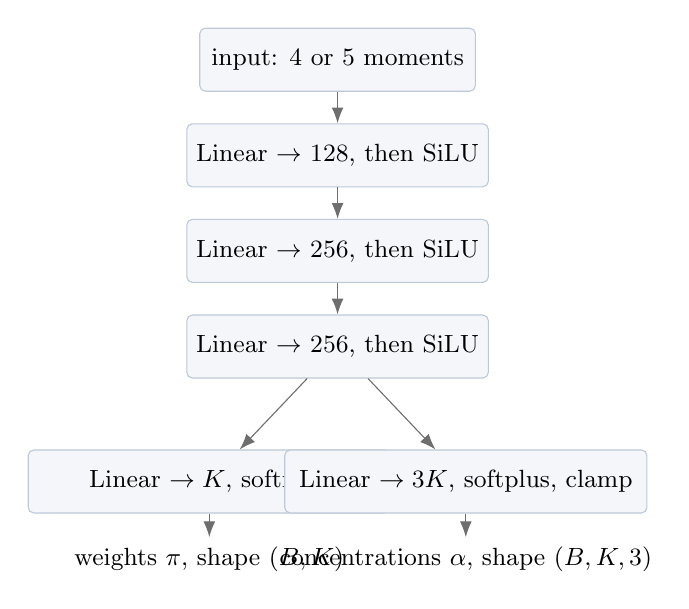
\begin{tikzpicture}[
  node distance=4mm,
  every node/.style={font=\small},
  layer/.style={draw=BoxRule, fill=BoxBG, rounded corners=2pt,
                minimum width=3.5cm, minimum height=8mm, align=center},
  head/.style={draw=BoxRule, fill=BoxBG, rounded corners=2pt,
               minimum width=4.6cm, minimum height=8mm, align=center},
  arrow/.style={-{Latex[length=2mm]}, draw=TagGray}
]
\node[layer] (in)  {input: 4 or 5 moments};
\node[layer, below=of in]  (l1) {Linear $\to$ 128, then SiLU};
\node[layer, below=of l1]  (l2) {Linear $\to$ 256, then SiLU};
\node[layer, below=of l2]  (l3) {Linear $\to$ 256, then SiLU};
\node[head, below left=9mm and -2.6cm of l3]  (hp) {Linear $\to K$, softmax};
\node[head, below right=9mm and -2.6cm of l3] (ha) {Linear $\to 3K$, softplus, clamp};
\node[below=3mm of hp, align=center] (op) {\small weights $\pi$, shape $(B,K)$};
\node[below=3mm of ha, align=center] (oa) {\small concentrations $\alpha$, shape $(B,K,3)$};
\draw[arrow] (in) -- (l1);
\draw[arrow] (l1) -- (l2);
\draw[arrow] (l2) -- (l3);
\draw[arrow] (l3) -- (hp);
\draw[arrow] (l3) -- (ha);
\draw[arrow] (hp) -- (op);
\draw[arrow] (ha) -- (oa);
\end{tikzpicture}
\end{center}

The shared stack of three layers is called the \term{trunk}, \Model{45}{self.trunk}. It turns
the handful of input moments into 256 internal numbers that both output heads can use. The two
heads then read those same 256 numbers and each produce a different part of the answer.

\paragraph{What a \term{Linear} layer does.} It multiplies its inputs by a matrix of learned
numbers and adds a learned offset. That is all --- it is a weighted sum.

\paragraph{What \term{SiLU} does.} If you stack linear layers directly, the whole stack
collapses into a single linear layer and can only represent straight-line relationships. You
need a \term{nonlinearity} between them. SiLU (also called Swish) is
$f(x) = x \cdot \sigma(x)$ where $\sigma$ is the S-shaped logistic curve. It passes large
positive values through nearly unchanged, squashes large negative values towards zero, and ---
unlike the older ReLU --- is smooth everywhere, which makes the training gradients better
behaved.

\section{The two output heads}

The two heads have different jobs, so they enforce different constraints.

\paragraph{Head $\pi$: the mixture weights.} \Model{52}{self.head\_pi} produces $K$ raw
numbers, which \code{torch.softmax} \ModelL{63} converts into $K$ non-negative numbers that sum
to 1:
\[
  \pi_k = \frac{e^{u_k}}{\sum_{j=1}^{K} e^{u_j}} .
\]
Exponentiating makes everything positive; dividing by the total makes them sum to one. So the
weights are valid by construction --- the network cannot produce an invalid answer even
before training.

\paragraph{Head $\alpha$: the concentrations.} \Model{53}{self.head\_alpha} produces $3K$ raw
numbers. These must be strictly positive, so they pass through \term{softplus},
$\mathrm{softplus}(x) = \log(1 + e^x)$, a smooth function that is always positive and
approaches $x$ for large $x$. Then:

\begin{itemize}
  \item A floor \code{alpha\_min} (default $1$) is added. Values below 1 create infinite
        density at an edge or corner. Because this implementation estimates each cell's
        mass from one density value at its centroid, it cannot integrate those singularities
        reliably. The constructor therefore rejects any floor below 1.
  \item A ceiling \code{alpha\_clip} (default $10^{3}$) is applied with \code{clamp}. Very
        large $\alpha$ means an extremely narrow spike, which produces enormous gradients and
        destabilises training.
  \item The flat vector of $3K$ numbers is reshaped to $(B, K, 3)$ so that component $k$ owns
        rows \code{alpha[:, k, :]}.
\end{itemize}

The constructor also validates its arguments up front \ModelL{32}: \code{n\_in} must be 4 or 5,
$K$ must be at least 1, the hidden width must be positive, the floor must be at least 1, and
the ceiling must exceed the floor.

\begin{caution}
This restriction is honest but important. The model cannot exactly represent a delta function,
an atom at a pure-stream corner, or probability living only on an edge. It can approximate
some narrow \emph{interior} peaks up to \code{alpha\_clip}, and those errors must be measured.
\end{caution}

\section{Size}

With $K = 16$, $\text{hidden} = 256$, and 5 input moments:
\[
  \underbrace{5{\cdot}128 + 128}_{\text{layer 1}} +
  \underbrace{128{\cdot}256 + 256}_{\text{layer 2}} +
  \underbrace{256{\cdot}256 + 256}_{\text{layer 3}} +
  \underbrace{256{\cdot}16 + 16}_{\text{head }\pi} +
  \underbrace{256{\cdot}48 + 48}_{\text{head }\alpha}
  \;\approx\; 116{,}000 \text{ parameters.}
\]
That is small enough to run inside an LES solver's inner loop, which was the point.

% ===================================================================
\chapter{How the Network Learns}
% ===================================================================

Training means adjusting those 116{,}000 numbers until the predictions match the data. What
counts as ``match'' is defined by the \term{loss} --- a single number, computed from a batch of
examples, that is small when the predictions are good. Training is then just: compute the
loss, work out which direction each parameter should move to reduce it, take a small step,
repeat.

The loss here is a sum of three parts \Loss{261}{combined\_loss}:
\[
  L_{\text{total}} \;=\; \underbrace{L_{\text{nll}}}_{\text{match the picture}}
  \;+\; \lambda_{\text{mom}} \underbrace{L_{\text{mom}}}_{\text{match the numbers}}
  \;-\; \lambda_{\text{ent}} \underbrace{H}_{\text{stay diverse}} .
\]

\section{Part 1: matching the histogram}
\label{sec:nll}

\Loss{80}{HistogramNLL} answers: ``if the true histogram were a bag of dots, how surprised
would my predicted formula be to see them?'' Lower surprise, better fit.

\subsection*{Precomputation in the constructor}

Everything that does not change from batch to batch is computed once when the module is
created \LossL{85}:

\begin{enumerate}
  \item Flatten the $64\times64$ grid and keep only cells with positive clipped area. Store
        each clipped polygon's centroid as \code{z\_simplex} of shape $(M, 3)$, with
        $z_3 = 1-z_1-z_2$.
  \item Store the cell areas of those $M$ cells, and their logarithms as \code{log\_cell\_area}.
  \item Store $\log$ of the normalised coordinates as \code{log\_z\_norm}, pre-shaped to
        $(1, M, 1, 3)$ so it can be broadcast against $\alpha$ without any reshaping at
        run time.
  \item Store the flat indices of the in-triangle cells, so a full $(B, 64, 64)$ histogram can
        be reduced to $(B, M)$ with one gather.
\end{enumerate}

All of these are registered as \code{buffers}, which means they automatically move to the GPU
when the model does but are not treated as trainable parameters.

\subsection*{The forward computation}

For a batch of $B$ examples \LossL{132}:

\begin{enumerate}
  \item \textbf{Log-density of every component at every cell.} Written out, the Dirichlet
        log-density is
        \[
          \log p(z_m \mid \alpha^{(k)}) = \sum_{i=1}^{3}(\alpha^{(k)}_i - 1)\log z_{m,i}
            \;-\; \sum_{i=1}^{3}\log\Gamma(\alpha^{(k)}_i)
            \;+\; \log\Gamma\!\Big(\sum_{i=1}^{3}\alpha^{(k)}_i\Big).
        \]
        The first term is a dot product against the precomputed \code{log\_z\_norm}; the other
        two are \code{lgamma} calls. Result shape: $(B, M, K)$.
  \item \textbf{Combine the components.} Add $\log \pi_k$ and use \code{logsumexp} over $k$:
        \[
          \log p(z_m) = \log \sum_k \pi_k\, p(z_m \mid \alpha^{(k)}) .
        \]
        \code{logsumexp} computes $\log \sum e^{x_i}$ without ever forming $e^{x_i}$, by
        factoring out the largest term. Doing it naively would overflow to infinity or
        underflow to zero within a few epochs.
  \item \textbf{Density to probability.} Multiply by the cell area --- in log space, add
        \code{log\_cell\_area}.
  \item \textbf{Renormalise over the triangle.} Subtract another \code{logsumexp}, this time
        over the cells. This is the crucial step: the true histogram sums to 1 over the
        triangle, so the prediction must too. Density-at-centroid times area is numerical
        quadrature, not an exact cell integral, so its raw sum is not exactly one.
  \item \textbf{Validate the target.} Reject non-finite values, negative values, zero total
        mass, or mass outside the clipped simplex. Then divide by the in-simplex total. This
        guarantees that every record contributes a normalized categorical target.
  \item \textbf{The surprise.} Multiply the normalized true histogram by the predicted log-probabilities,
        sum, and negate:
        \[
          L_{\text{nll}} = -\frac{1}{B}\sum_{b=1}^{B}\sum_{m=1}^{M} p_{b,m} \log q_{b,m} .
        \]
\end{enumerate}

\begin{analogy}
Imagine the true histogram is a list of guesses people made, and the prediction is a bookie's
odds. This loss is the total ``I can't believe that happened'' score. Good odds give a low
score.
\end{analogy}

\subsection*{An optimisation worth knowing about}

The forward pass accepts either a full $(B, 64, 64)$ histogram or an already-flattened
$(B, M)$ one \LossL{148}, deciding by checking the tensor's shape. If you pass
\code{--flat-histograms} on the training command line, the dataset does the flattening once
at load time \DataL{182} and the loss skips a reshape-and-gather on every single batch.

\section{Part 2: encouraging the moments to match}

The histogram loss cares about the whole picture. But we also want the prediction's mean and
variance to agree with the numbers we fed in. The loss encourages agreement, but does not solve
an equation that forces exact agreement.

The wonderful thing about a Dirichlet mixture is that its moments can be computed by algebra,
with no sampling and no integration. \Loss{165}{mixture\_moments} does it in nine lines.

Per component $k$, with $\alpha_0^{(k)} = \sum_i \alpha^{(k)}_i$:
\[
  \mu^{(k)}_i = \frac{\alpha^{(k)}_i}{\alpha_0^{(k)}}, \quad
  v^{(k)}_i = \frac{\mu^{(k)}_i (1 - \mu^{(k)}_i)}{\alpha_0^{(k)} + 1}, \quad
  c^{(k)}_{12} = \frac{-\alpha^{(k)}_1\alpha^{(k)}_2}{\big(\alpha_0^{(k)}\big)^2\big(\alpha_0^{(k)} + 1\big)} .
\]

Combining them across the mixture needs care. The mean is a simple weighted average:
\[
  \mathbb{E}[Z_i] = \sum_k \pi_k\, \mu^{(k)}_i .
\]
But the \emph{variance} is not. You cannot just average the component variances, because the
components sit in different places and that separation is itself a source of spread. The
correct route is via the second moment:
\[
  \mathbb{E}[Z_i^2] = \sum_k \pi_k\Big(v^{(k)}_i + \big(\mu^{(k)}_i\big)^2\Big),
  \qquad
  \mathrm{Var}[Z_i] = \mathbb{E}[Z_i^2] - \big(\mathbb{E}[Z_i]\big)^2 .
\]
And likewise for the covariance:
\[
  \mathbb{E}[Z_1 Z_2] = \sum_k \pi_k\Big(c^{(k)}_{12} + \mu^{(k)}_1\mu^{(k)}_2\Big),
  \qquad
  \mathrm{Cov}[Z_1, Z_2] = \mathbb{E}[Z_1 Z_2] - \mathbb{E}[Z_1]\mathbb{E}[Z_2] .
\]

\begin{analogy}
Two rifle groupings, each tight, but centred a metre apart. The combined spread is far larger
than either group's own spread, because you must also account for the gap between them. That
gap is the $-(\mathbb{E}[Z])^2$ correction.
\end{analogy}

\Loss{206}{stack\_predicted\_moments} arranges these into the same order as the input vector
--- $[\mathbb{E}_1, V_1, \mathbb{E}_2, V_2]$ for the four-moment setting, with
$\mathrm{Cov}_{12}$ appended for five. Before squaring errors, \code{moment\_loss} divides
mean errors by 1 and variance/covariance errors by 0.25, their natural physical ranges:
\[
  L_{\rm mom} = \operatorname{mean}_j
  \left(\frac{\widehat m_j-m_j}{s_j}\right)^2,\qquad
  s=[1,0.25,1,0.25,0.25].
\]
This makes the errors dimensionless, so the smaller-valued variances and covariance are not
ignored merely because of their numerical scale.

This term is weighted by \code{--lambda-mom} (default 0.5).

\begin{caution}
The moments can be computed exactly \emph{from the predicted parameters}; this does not mean
they equal the conditioning moments exactly. Evaluation reports absolute and relative errors.
A solver should not use a model whose measured errors exceed its physical tolerance.
\end{caution}

\begin{caution}
Note carefully that the moment loss compares against the \emph{unscaled} moments, while the
network sees \emph{scaled} moments as input. Look at the training inner loop \TrainL{327}: the
scaler is applied to make \code{m\_scaled} for the model, but the raw \code{moments} tensor is
what is passed to the loss. Mixing these up would make the moment term meaningless.
\end{caution}

\section{Part 3: keeping the components alive}

Mixture models have a well-known failure mode: the optimiser discovers that it can drive most
of the weights $\pi_k$ to nearly zero and do all the work with two or three components. The
other thirteen become dead weight, and the model is effectively much less expressive than you
paid for.

The cure is to reward spread-out weights. \Loss{222}{entropy\_reg} computes
\[
  H = \frac{1}{B}\sum_{b=1}^{B}\left(-\sum_{k=1}^{K}\pi_{b,k}\log \pi_{b,k}\right),
\]
which is largest when all weights are equal and zero when one weight takes everything. Because
we want $H$ \emph{large} and the optimiser always makes the total \emph{small}, the term enters
the sum with a minus sign \LossL{269} --- that is, we minimise $-\lambda_{\text{ent}} H$.

The default weight \code{--lambda-ent} is $10^{-3}$: a gentle nudge, not a hard rule. Push it
too high and every component is forced to be equally important whether or not that helps.

\section{Numerical hygiene throughout}

Three habits recur in the loss code and are worth internalising:

\begin{itemize}
  \item \textbf{Everything in logarithms.} Probabilities multiply; logarithms add. Adding is
        numerically stable, multiplying tiny numbers is not.
  \item \textbf{\code{logsumexp} instead of \code{log(sum(exp(...)))}.} See
        \Loss{50}{mixture\_logpdf} and the inline version at \LossL{144}.
  \item \textbf{Small constants everywhere.} \code{LOG\_EPS} $= 10^{-12}$ \LossL{30} guards
        $\log \pi$; \code{eps} $= 10^{-7}$ guards $\log z$ inside
        \Loss{37}{dirichlet\_logpdf}. Without them the very first batch containing an empty
        histogram cell yields \code{NaN} and the run is dead.
\end{itemize}

% ===================================================================
\chapter{Feeding the Network: Dataset and Splits}
\label{ch:splits}
% ===================================================================

\section{The dataset adapter}

\Data{76}{HybridPDFDataset} is the bridge between the files on disk and the training loop. Its
guiding principle, stated in the module docstring, is \term{schema tolerance}: it accepts
metadata written by either the old or the new version of the writer.

\Data{48}{load\_metadata} handles this by looking for \code{run\_id} \emph{or}
\code{run\_number}, and \code{box\_width} \emph{or} \code{filter\_width}, renaming whichever it
finds to the canonical name, then verifying that all twelve required columns are present and
raising a clear error listing exactly which are missing if not.

\subsection*{A safety check you should not skip}

On construction, the dataset rebuilds the bin grid from
scratch using \Grid{75}{bin\_grid} and compares it against the \code{/bins} group actually
stored in a shard, including clipped areas, clipped centroids, and the mask.

This matters because the training code re-derives the grid from three numbers
(\code{--num-bins}, \code{--zst}, \code{--uniform-bins}) rather than reading it from the file.
If you train with the wrong $z_{\text{st}}$, every histogram would be silently misinterpreted
and the results would be quietly wrong. The check turns a silent disaster into a loud crash.

Training additionally runs \code{validate\_dataset} over \emph{every} shard and record before
the first epoch. It checks file presence, shapes, finite non-negative masses, normalization,
zero mass outside the simplex, one-to-one Parquet-to-HDF5 row mappings, stored sample IDs, and
the difference between moments computed from raw DNS values and from histograms. The default
maximum allowed moment discrepancy is 0.05. A JSON copy of the validation result is saved in
the run directory.

\begin{caution}
Files generated by the old centre-masked writer do not contain clipped centroids and use a
different meaning for cell area. The validator rejects them. They must be regenerated; silently
``upgrading'' only their metadata would not restore probability mass already discarded.
\end{caution}

\subsection*{Fetching one example}

\Data{162}{\_\_getitem\_\_} does the following:

\begin{enumerate}
  \item Look up the row: which shard file, which row inside it.
  \item Open the shard lazily. Handles are cached in a dictionary \DataL{136}, so the file is
        opened at most once even across hundreds of thousands of reads.
  \item Read the histogram.
  \item Verify every fetched histogram is finite, non-negative, and sums to 1.
  \item Optionally flatten to in-triangle cells; optionally store in a RAM cache.
  \item Assemble the 4- or 5-element moment vector and the metadata dictionary.
\end{enumerate}

\subsection*{Two speed options}

\code{--cache-histograms} keeps every histogram in memory after its first read. The help text
quotes about 2.6~GB for the full dataset. Since training runs hundreds of epochs, this turns
hundreds of passes over compressed disk data into one.

\code{--flat-histograms} stores only the in-triangle cells, roughly halving both memory and
per-batch work. Used together, the two options remove file input/output from the training loop
almost entirely.

\subsection*{Batching}

\Data{224}{collate\_records} stacks a list of examples into batched tensors and converts the
metadata into parallel tensors, keeping \code{scalar\_config} as a plain list of strings since
it is text.

\section{Making an honest train/test split}

This is the part that decides whether your reported accuracy means anything.

\subsection*{The leakage trap}

Suppose you shuffled all 165{,}895 examples and took 15\% at random for testing. Two examples
from overlapping windows of the same snapshot are nearly identical --- one would land in
training and its near-twin in testing. Your test score would be excellent and completely
meaningless, because you would only have proved that the network can recognise things it has
already seen.

\subsection*{The fix: one global split by simulation run}

\code{make\_split} splits by \code{run\_id}, not by row. All examples from run~7 go
entirely into training, or entirely into validation, or entirely into testing. Since different
runs start from different random initial conditions, a test run is genuinely unseen physics.

The run list is shuffled once with a recorded seed and partitioned once for the whole dataset.
It is \emph{not} partitioned separately for each scalar configuration, because those
configurations can share the same underlying velocity realization.

\begin{itemize}
  \item Default ratios are 70/15/15. Requested zero ratios remain exactly zero. With too few
        runs to populate every nonzero partition, a partition may be empty; the code never
        falls back to splitting one run by timestep.
  \item If \code{--holdout-config} names a configuration, that entire configuration becomes the
        test set and everything else is split 80/20 between training and validation. This is
        specifically a configuration-generalization test. It is allowed only when the held
        configuration uses run IDs absent from every other configuration. If run IDs are
        shared, the program stops: keeping the test set pure, covering every row, and keeping
        a physical run in one partition cannot all be satisfied at once.
\end{itemize}

The saved split includes exact indices, run lists, grouping policy, and a SHA-256 fingerprint
of the ordered metadata. Loading checks that indices are unique, in range, mutually disjoint,
cover every row exactly once, obey holdout rules, and match the current dataset fingerprint.
Thus a split file from a different Parquet dataset is rejected even if its row count happens
to match.

You can inspect a split before committing to it with
\code{python -m dirichlet\_mdn.preview\_split}, which writes a Markdown table and a CSV
summary; see \code{splits/by\_run\_id\_seed0/} in this workspace for an example.

% ===================================================================
\chapter{The Training Loop}
% ===================================================================

\section{Setup}

\Train{213}{train} performs, in order:

\begin{enumerate}
  \item Seed every random number generator so the run is reproducible.
  \item Create a run directory named with a UTC timestamp down to microseconds, your
        \code{--tag}, and a random suffix. Existing directories are never reused.
  \item Load and exhaustively validate the dataset.
  \item Either build a split or load and verify a pre-computed one from
        \code{--splits-json}.
  \item \textbf{Fit the input scaler} \TrainL{265} on the \emph{training rows only}.
  \item Build the model, the loss module, and the data loaders.
  \item Create the optimiser and the learning-rate schedule.
\end{enumerate}

\subsection*{Why scale the inputs, and why a robust scaler}

The five moments live on wildly different scales: means are around $0.1$--$0.9$, variances
around $0.001$--$0.05$, covariance can be negative. A neural network trained on such
mismatched inputs converges slowly, because the same step size is far too big for one input
and far too small for another.

The fix is to standardise each input. This code uses scikit-learn's \code{RobustScaler}, which
subtracts the \emph{median} and divides by the \emph{interquartile range} (the width of the
middle 50\% of the data), rather than the more common mean-and-standard-deviation. The reason
is outliers: a handful of extreme variance values would badly distort a mean-based scaler,
while the median barely notices them.

\Train{105}{TorchScaler} wraps the fitted scaler so it can be applied directly to a GPU tensor,
avoiding a round trip to the CPU on every batch. It also guards against division by zero by
replacing any scale below $10^{-6}$ with 1.0 \TrainL{114}.

\begin{caution}
The scaler is fitted on training rows only, then applied unchanged to validation and test rows.
Fitting on the full dataset would leak information about the test distribution into training.
The exact centre and effective scale used by PyTorch are saved in
\code{input\_transform.json}. Evaluation loads that language-independent file. The older
\code{scaler.pkl} is retained for inspection, but is not the deployment contract.
\end{caution}

\section{The optimiser and the schedule}

\TrainL{292} creates \code{AdamW}. In plain terms, Adam keeps a running memory of both the
recent direction of improvement and the recent size of the changes, and uses them to give each
parameter its own effective step size. The ``W'' variant additionally applies
\term{weight decay} --- a gentle pull of every parameter towards zero --- in the mathematically
correct way. Weight decay discourages the network from relying on any single huge parameter,
which usually improves generalisation. Defaults: learning rate $3 \times 10^{-4}$, weight decay
$10^{-5}$.

\TrainL{293} adds \code{CosineAnnealingLR}. The learning rate starts at its full value and
follows a cosine curve down to nearly zero by the last epoch. Big steps early explore the
landscape; tiny steps late settle precisely into a minimum.

\section{One epoch}

An \term{epoch} is one complete pass over the training data. For each batch, starting at
\TrainL{314}:

\begin{enumerate}
  \item Move the moments and the histogram to the compute device.
  \item Apply the scaler to produce \code{m\_scaled}.
  \item Forward pass: \code{pi, alpha = model(m\_scaled)} \TrainL{327}.
  \item Compute the three-part loss against the \emph{raw} moments and the true histogram.
  \item Zero the accumulated gradients, then back-propagate \code{loss.total}.
  \item \textbf{Clip the gradients} to a maximum overall length of \code{--grad-clip}
        (default 5.0) \TrainL{334}. Occasionally a pathological batch produces an enormous
        gradient that would throw the parameters into nonsense; clipping caps the step size
        while preserving its direction.
  \item Take one optimiser step.
  \item Every \code{--log-every-n-batches} batches (default 25), print progress.
\end{enumerate}

After the batches, step the learning-rate schedule and run
\Train{133}{evaluate\_loss} over the validation set with gradients disabled.

\section{Choosing when to stop}

\begin{itemize}
  \item \textbf{Best-model tracking.} By default, if the full validation loss improves,
        \code{model\_best.pt} is rewritten. This matches the objective actually optimized,
        including moment and entropy terms. \code{--selection-metric nll} is available for an
        explicitly likelihood-only experiment.
  \item \textbf{Early stopping.} A counter tracks epochs without improvement. When it reaches
        \code{--patience} (default 30), training halts \TrainL{421}. Set patience to 0 to
        disable.
  \item \textbf{Last-model checkpoint.} \code{model\_last.pt} is always written too, so you can
        inspect the end state even if it overfitted.
\end{itemize}

\section{What a run directory contains}

\begin{center}
\begin{tabular}{@{}ll@{}}
\toprule
\textbf{File} & \textbf{Contents} \\
\midrule
\code{manifest.json} & Every configuration value, dataset statistics, split totals, best score \\
\code{dataset\_validation.json} & Result of checking every dataset row and shard \\
\code{splits.json}   & The exact row indices of each split, plus the provenance description \\
\code{input\_transform.json} & Exact centre and scale required to use the model \\
\code{scaler.pkl}    & Original fitted scikit-learn object, retained for inspection \\
\code{model\_best.pt} & Weights at the best configured validation metric \\
\code{model\_last.pt} & Weights at the final epoch \\
\code{tb/}            & TensorBoard event files for live curves \\
\code{train.log}      & Per-epoch loss table, also echoed to the terminal \\
\bottomrule
\end{tabular}
\end{center}

New manifests declare artifact schema version~2. Older run directories predate these checks
and should not be treated as validated under the corrected pipeline. They are rejected by
default. For historical comparison only, \code{evaluate --allow-legacy-artifacts} loads the
grid stored in their HDF5 file and their older \code{scaler.pkl}; it emits a warning because
those metrics are not directly comparable with clipped-grid version-2 results. The option is
explicit because pickle files must only be loaded from a trusted run directory.

\section{Devices}

\Train{90}{resolve\_device} maps \code{--device auto} to an NVIDIA GPU if present, otherwise to
Apple Silicon's Metal backend, otherwise to the CPU. Because the model is tiny, CPU training is
perfectly viable for small experiments.

% ===================================================================
\chapter{Judging the Result}
\label{ch:eval}
% ===================================================================

\section{Turning parameters back into a picture}

\Metric{28}{predict\_histograms} does the reverse of the loss: given $\pi$ and $\alpha$, it
evaluates the mixture at every in-triangle cell, multiplies by cell area, renormalises, and
returns a $(B, 64, 64)$ array directly comparable with the stored histogram. Cells outside the
triangle are left at zero.

\section{The measurements that matter}

\begin{description}[leftmargin=1.6cm, style=nextline]
  \item[Test negative log-likelihood] The same normalized categorical surprise used for
        training, now reported separately for every held-out record. This answers whether
        the model assigned probability where the DNS actually placed it.
  \item[$L_1$ error] \Metric{72}{joint\_l1} sums the absolute cell-by-cell differences,
        $\sum_{ij} |p_{ij} - q_{ij}|$, over the triangle. Because both tables sum to 1, this
        ranges from 0 (identical) to 2 (no overlap at all). Half of it is the fraction of
        probability mass sitting in the wrong place --- an $L_1$ of 0.2 means 10\% of the mass
        is misplaced. It is the easiest metric to explain to a non-specialist.
  \item[Jensen--Shannon divergence] \Metric{79}{joint\_jsd} is the same family of measure used
        in the sampler, computed here in \emph{bits} (base-2 logarithms) to match the
        convention in the legacy \code{MLPDF.py}. It ranges from 0 to 1 bit. Unlike $L_1$ it is
        sensitive to relative errors, so it notices when a region that should have a small
        amount of probability has none at all.
  \item[Marginal divergences] \Metric{92}{marginal\_jsd} collapses the two-dimensional
        histogram onto one axis (summing over the other) and compares those one-dimensional
        profiles. This separates ``is scalar~A right on its own?'' from ``is the relationship
        between A and B right?''. A model can score well on both marginals and still get the
        joint structure wrong.
  \item[Moment recovery error] \Metric{125}{moment\_recovery\_error} compares the closed-form
        moments of the prediction against the input moments, absolutely and relatively. This is
        the physics constraint: if it is not near zero, the prediction is not usable in a solver
        regardless of how good the picture looks. The evaluator also divides by the physical
        scales $[1,0.25,1,0.25,0.25]$ and compares the worst result with
        \code{--moment-acceptance-tolerance} (default 0.05), writing an explicit pass/fail field.
\end{description}

\Metric{120}{mixture\_active\_count} additionally counts how many components carry weight above
1\% --- the direct diagnostic for the component-collapse problem the entropy term was designed
to prevent. If you train with $K = 16$ and this consistently reports 3, you are paying for
capacity you are not using.

\section{Slicing the results}

Aggregate numbers hide problems. \Metric{149}{per\_config\_breakdown} and
\Metric{168}{per\_timestep\_breakdown} report mean, standard deviation, and count for every
metric, grouped by scalar configuration and by configuration-and-timestep. This is how you
discover that the model is excellent everywhere except one configuration, or that accuracy
degrades steadily as the flow mixes.

The JSON summary distinguishes three averages. A \term{micro average} gives every retained
record one vote. A \term{macro average} first averages within each configuration and then gives
each configuration one vote. A \term{source-weighted average} uses the inverse retention
weights written by the sampler. Standard deviations are reported alongside micro and macro
means. These views are all necessary because deliberate diversity selection makes the retained
dataset unbalanced.

\begin{caution}
The proposal also asks for a downstream reaction-rate or closure error. That quantity requires
a reaction-rate function or chemistry table, neither of which this repository supplies.
The evaluator therefore does \emph{not} invent one. No claim about LES reaction-rate accuracy
should be made until that external physical definition and a corresponding held-out metric are
added.
\end{caution}

\Eval{206}{evaluate\_run} runs the whole pipeline and writes
\code{metrics\_per\_record.csv}, \code{metrics\_per\_config.csv},
\code{metrics\_per\_config.md}, \code{metrics\_per\_timestep.csv}, and
\code{eval\_summary.json} into an \code{eval/} subdirectory, plus a folder of plots.

\section{The plots}

\begin{itemize}
  \item \Plot{46}{plot\_pdf\_comparison} divides probability mass by clipped cell area and puts
        the true and predicted \emph{densities} side by side using the actual non-uniform bin
        edges and a shared colour scale. It overlays the triangle boundary via
        \Plot{30}{\_add\_simplex\_overlay}. This is the plot to look at first --- your eye will
        catch structural errors that no single number reports.
  \item \Plot{84}{plot\_metric\_vs\_timestep} draws error against time, one line per
        configuration, revealing whether the model degrades as mixing proceeds.
  \item \Plot{108}{plot\_alpha\_diagnostics} shows the distribution of active component counts
        and a log-scale scatter of overall concentration against variance.
  \item \Plot{145}{plot\_moment\_recovery} scatters predicted against target for each moment
        with a $y = x$ reference line. Points off the diagonal are constraint violations.
  \item \Plot{171}{write\_pdf\_album} bundles a selection into a single multi-page PDF for
        review.
\end{itemize}

% ===================================================================
\chapter{Built-In Self-Checks}
% ===================================================================

\code{dirichlet\_mdn/verify.py} contains five tests designed to catch the specific mistakes
that are easy to make and hard to notice. Run them with \code{pixi run verify} before trusting
any result.

\begin{enumerate}
  \item \Verify{43}{check\_bins} --- Rebuild the bin grid from the three parameters and compare
        against a stored shard, to $10^{-9}$. Catches a wrong $z_{\text{st}}$ or bin count,
        which would silently misinterpret every histogram.
  \item \Verify{54}{check\_loss\_gradient} --- Push eight real examples forward and backward and
        confirm the loss and every gradient are finite. Catches numerical blow-ups before you
        waste hours on a training run that will produce \code{NaN}.
  \item \code{check\_moments\_against\_monte\_carlo} --- Draw 400{,}000 samples with
        NumPy's independent Dirichlet random generator and compare empirical means, variances,
        and covariance with the model formulas. This avoids the circular mistake of generating
        a target with the same helper being tested.
  \item \Verify{98}{check\_permutation\_invariance} --- Shuffle the order of the $K$ components
        and confirm the loss is unchanged to within $10^{-6}$. The components are unordered by
        definition; if relabelling them changed the answer, there would be an indexing bug.
  \item \Verify{166}{check\_k1\_fits\_analytical\_dirichlet} --- Generate 750{,}000 independent
        NumPy samples from a known single Dirichlet, bin those samples, fit a $K=1$ model, and
        compare recovered parameters with the truth. The target is no longer produced by the
        same density routine that is under test.
\end{enumerate}

The separate \code{pixi run test} command runs deterministic \code{unittest} regressions for
clipped geometry, scalar validation, global split isolation and fingerprints, concentration
bounds, target normalization, diagnostic labels, exact preprocessing artifacts, and MPI rank
provenance.

% ===================================================================
\chapter{Running Everything}
% ===================================================================

\section{Setting up the environment}

The workspace ships a \code{pixi.toml} at its root. \code{pixi} is an environment manager: it
reads that file, downloads exactly the listed packages, and gives you an isolated environment.
Nothing is installed system-wide and nothing conflicts with your other projects.

\begin{center}
\begin{tabular}{@{}ll@{}}
\toprule
\textbf{Command} & \textbf{Effect} \\
\midrule
\code{pixi install} & Create the environment (first time only) \\
\code{pixi shell}   & Drop into a shell with everything on the path \\
\code{pixi task list} & List every available task \\
\code{pixi run <task>} & Run one task \\
\bottomrule
\end{tabular}
\end{center}

The environment includes NumPy, pandas, PyArrow, h5py, SciPy, scikit-learn, matplotlib,
PyTorch, TensorBoard, \code{mpi4py} with OpenMPI, and \code{tectonic} for building this
document.

\section{The task list}

\begin{longtable}{@{}lp{10.2cm}@{}}
\toprule
\textbf{Task} & \textbf{What it does} \\
\midrule
\endhead
\code{sample-mpi <n>}   & Full MPI sampling with $n$ processors. Both phases.
                          Example: \code{pixi run sample-mpi 52} \\
\code{sample-mpi-smoke} & Two processors, two runs, one timestep --- a quick plumbing test \\
\code{merge-only}       & Re-run Phase 2 over an existing \code{\_rank/} tree. No MPI needed \\
\code{sample-serial}    & The single-process reference sampler \\
\code{verify}           & The five self-checks \\
\code{test}             & Deterministic regression tests for the accuracy corrections \\
\code{diversity}        & Dataset coverage audit with plots \\
\code{preview-split <seed>} & Build and report a split without training \\
\code{train <K> <M> <epochs> <tag>} & Train the network.
                          Example: \code{pixi run train 16 5 500 mdn\_K16} \\
\code{train-smoke}      & Two epochs, to confirm the loop runs \\
\code{evaluate <dir>}   & Full evaluation of a finished run \\
\code{tensorboard}      & Live training curves in a browser \\
\code{doc}              & Rebuild this document with tectonic \\
\bottomrule
\end{longtable}

The default paths are set in the \code{[activation.env]} block of \code{pixi.toml}
(\code{DNS\_ROOT}, \code{PARQUET}, \code{HDF5\_DIR}, \code{RUNS\_DIR}). Edit them there rather
than retyping long paths.

\section{A recommended first session}

\begin{enumerate}
  \item \code{pixi install}
  \item \code{pixi run test} --- run deterministic regression tests
  \item \code{pixi run verify} --- confirms the existing dataset and the code agree
  \item \code{pixi run diversity} --- look at what is actually in the dataset
  \item \code{pixi run preview-split 0} --- see which runs go where
  \item \code{pixi run train-smoke} --- two epochs, confirm the loop works
  \item \code{pixi run train 16 5 500 my\_first\_run} --- the real thing
  \item \code{pixi run tensorboard} --- watch it learn
  \item \code{pixi run evaluate dirichlet\_mdn\_runs/<timestamp>\_my\_first\_run}
\end{enumerate}

\section{Practical notes on the MPI sampler}

\begin{itemize}
  \item There are only 216 work units, so more than 216 processors buys nothing.
  \item Phase~1 keeps every candidate on disk but buffers only one shard per rank. Lower
        \code{--hdf5-shard-size} to trade more files for less memory. Phase~2 similarly bounds
        metadata with \code{--merge-sort-chunk-rows}; temporary sorted Parquet files require
        additional disk space until the merge finishes.
  \item Always pass \code{--keep-rank-outputs} on a long run. Re-running the merge afterwards
        with \code{--skip-phase1} is minutes; re-running Phase~1 is days.
  \item Phase 2 is single-threaded by construction. On the production dataset it took about
        three hours. Watch the progress lines to confirm it is moving.
  \item Read the manifest's \code{missing\_paths} before using the dataset.
\end{itemize}

% ===================================================================
\chapter{Accuracy Review: What Changed and What Did Not}
% ===================================================================

This chapter is a short map for a new reader who encounters an older dataset, split, or run
directory. The September 2026 review found that several checks agreed with each other while
still sharing the same mistaken assumption. The corrections therefore changed the stored data
format to version~2; old generated data must be rebuilt.

\begin{longtable}{@{}p{3.2cm}p{5.2cm}p{6.0cm}@{}}
\toprule
\textbf{Area} & \textbf{Old risk} & \textbf{Corrected behavior} \\
\midrule
\endhead
Serial sampling & Two incompatible programs occupied one file. &
The serial command calls the canonical MPI implementation with one rank. \\
Triangle boundary & A rectangle was kept or dropped by its centre. &
Every rectangle is clipped; its true intersection area and centroid are stored. \\
Scalar values & Invalid values could disappear during histogramming. &
Values are checked, tiny round-off is counted and corrected, and every used pair must be counted. \\
MPI selection & Each rank discarded candidates before the global decision. &
Phase~1 is lossless; Phase~2 checks provenance and sees every candidate in seeded hash order. \\
Splits & Scalar configurations could put one physical run in different partitions. &
Ordinary experiments partition the global run list once, and split files carry a dataset fingerprint. \\
Training data & Only a small sample of file integrity was checked. &
Training checks every shard, mapping, histogram, geometry array, and moment discrepancy first. \\
Moment claim & A penalty was described as an exact constraint. &
The penalty is dimensionless, total loss selects checkpoints by default, and measured errors get a pass/fail tolerance. \\
Plots & Unequal-bin probability mass was drawn as though it were density. &
Plots divide mass by clipped area and use the actual bin edges. \\
Verification & Some targets were generated by the same formula being tested. &
NumPy Monte Carlo samples provide independent moment and recovery references. \\
\bottomrule
\end{longtable}

\section{Deliberate deviations and remaining limits}

\begin{enumerate}
  \item \textbf{No singular boundary integration.} A full plan could numerically integrate
        Dirichlet densities with $\alpha<1$ inside every clipped cell. The implementation instead
        requires $\alpha\geq1$. This is simpler and stable, but cannot represent exact edge or
        corner atoms.
  \item \textbf{Lossless extraction needs temporary disk space.} Local pruning was removed.
        Incremental shards and external metadata sorting now bound memory, but Phase~1 files
        plus temporary sort runs must fit on disk.
  \item \textbf{No invented chemistry score.} Test NLL and PDF/moment errors are implemented.
        Reaction-rate error is not, because no chemistry function or table is available here.
  \item \textbf{No silent conversion of old data.} Version-1 histograms may already have lost
        boundary mass. Version~2 rejects them and requires regeneration.
  \item \textbf{No real-DNS accuracy result is implied by unit tests.} Synthetic tests verify
        logic. Production acceptance still requires regenerating the private DNS-derived data,
        running MPI rank-count/seed studies, training, and evaluating held-out runs.
\end{enumerate}

\begin{plainbox}{The practical rule}
Trust a result only when \code{pixi run test} passes, the run contains
\code{dataset\_validation.json} and \code{input\_transform.json}, the split fingerprint matches,
the evaluation's moment acceptance field passes, and the relevant held-out PDF metrics are
reported. Even then, a separate reaction-rate test is required before claiming LES closure
accuracy.
\end{plainbox}

% ===================================================================
\chapter*{Glossary}
\addcontentsline{toc}{chapter}{Glossary}
% ===================================================================

\begin{description}[leftmargin=3.4cm, style=nextline, font=\normalfont\bfseries]
  \item[Barrier] A synchronisation point where every processor waits until all have arrived.
  \item[Batch] A group of examples processed together in one training step.
  \item[Bimodal] Having two separate peaks.
  \item[Bin] One small rectangle of the histogram grid.
  \item[Covariance] A measure of whether two quantities vary together.
  \item[Dirichlet distribution] A probability distribution over the triangle, controlled by
        three positive numbers.
  \item[DNS] Direct Numerical Simulation: the fine, expensive reference simulation.
  \item[Early stopping] Halting training when validation performance stops improving.
  \item[Entropy] A measure of how spread out a set of probabilities is.
  \item[Epoch] One complete pass over the training data.
  \item[Filter box] A cube of DNS cells treated as one coarse cell.
  \item[Gradient] The direction and rate at which the loss changes as a parameter changes.
  \item[HDF5] A file format for large numeric arrays.
  \item[Histogram] A table of counts (here, fractions) per bin.
  \item[Jensen--Shannon distance] A symmetric, bounded measure of how different two
        distributions are.
  \item[LES] Large Eddy Simulation: the coarse, affordable simulation.
  \item[Linear layer] A learned weighted sum plus an offset.
  \item[Logsumexp] A numerically safe way to compute $\log \sum e^{x_i}$.
  \item[Loss] The single number training tries to minimise.
  \item[MDN] Mixture Density Network: a network that outputs the parameters of a mixture
        distribution.
  \item[Mean] The average.
  \item[Mixture] A weighted sum of several distributions.
  \item[Moments] The summary numbers: means, variances, covariance.
  \item[MPI] Message Passing Interface: the standard for multi-processor programs.
  \item[NLL] Negative log-likelihood: the ``surprise'' score.
  \item[Parquet] A columnar table file format built for fast queries.
  \item[Periodic] Wrapping around at the boundaries, like an infinite tiled pattern.
  \item[PDF] Probability density function: the shape of a distribution.
  \item[Rank] A processor's identity number in an MPI job, from 0 upwards.
  \item[Shard] One file of a dataset split across several files.
  \item[Simplex] The triangle of allowed values.
  \item[Softmax] A function turning arbitrary numbers into positive numbers summing to 1.
  \item[Softplus] A smooth function that is always positive.
  \item[Stride] How far the sliding window moves between samples.
  \item[Variance] A measure of spread.
  \item[Weight decay] A gentle pull of parameters towards zero, to improve generalisation.
\end{description}

% ===================================================================
\chapter*{Appendix: Index of Source Locations}
\addcontentsline{toc}{chapter}{Appendix: Index of Source Locations}
% ===================================================================

\section*{\code{EnsightPDFHybridDatasetMPI.py} --- the MPI sampler}

\begin{longtable}{@{}rp{4.9cm}p{7.3cm}@{}}
\toprule
\textbf{Line} & \textbf{Name} & \textbf{Role} \\
\midrule
\endhead
41   & \code{SCALAR\_CONFIGS} & The eight configuration labels \\
42   & \code{MOMENT\_NAMES} & The five moment column names \\
43   & \code{SHAPE\_NAMES} & The ten shape feature names \\
57   & \code{parse\_int\_spec} & Parses \code{0:27} or \code{0,3,5} into a list \\
80   & \code{parse\_str\_list} & Parses a comma-separated string list \\
87   & \code{fill\_periodic} & Wraps the cube with periodic ghost cells \\
104  & \code{read\_ensight} & Reads and un-decomposes the two binary files \\
149  & \code{get\_bin\_centers} & Non-uniform bin centre placement \\
177  & \code{get\_histogram\_layout} & Edges, centres, areas, triangle mask \\
215  & \code{compute\_direct\_moments} & Five moments from raw values \\
224  & \code{compute\_histogram\_pdf} & Counts into bins, normalises to 1 \\
237  & \code{compute\_histogram\_moments} & Five moments from the histogram \\
246  & \code{build\_shape\_masks} & Seven regional stencils \\
264  & \code{compute\_shape\_features} & Ten shape descriptors \\
286  & \code{jensen\_shannon\_distance} & Distance between two histograms \\
297  & \code{js\_distance\_to\_stack} & One against many, vectorised \\
323  & \code{pairwise\_min\_distances} & Nearest-neighbour distance within a set \\
349  & \code{compute\_moment\_bin} & Five moments to a five-integer bin key \\
369  & \code{min\_distance\_to\_existing} & Scalar loop version of the above \\
376  & \code{get\_existing\_novelties} & Per-item novelty, scalar version \\
388  & \code{decide\_retention} & The four-way keep/replace/discard rule \\
414  & \code{iter\_filter\_records} & The sliding-window generator \\
462  & \code{write\_hdf5\_shards} & Writes histograms and bin definition \\
503  & \code{remove\_existing\_shards} & Cleans stale output files \\
513  & \code{build\_metadata\_frame} & Builds the Parquet table \\
533  & \code{materialize\_dataset} & Writes HDF5 + Parquet + manifest \\
591  & \code{build\_arg\_parser} & All command-line options \\
628  & \code{enumerate\_work\_units} & All (run, configuration) pairs \\
636  & \code{partition\_work\_units} & Round-robin deal to processors \\
640  & \code{process\_work\_units\_on\_rank} & Phase 1: lossless per-processor extraction \\
766  & \code{write\_rank\_outputs} & Phase 1 output, including empty manifests \\
831  & \code{iter\_rank\_candidates} & Fast streaming read-back of candidates \\
881  & \code{merge\_per\_rank\_outputs} & Phase 2: global merge with novelty cache \\
1024 & \code{aggregate\_rank\_manifests} & Sums counters, collects missing paths \\
1047 & \code{main} & MPI setup, phase orchestration, final write \\
\bottomrule
\end{longtable}

\section*{\code{dirichlet\_mdn/} --- the neural network package}

\begin{longtable}{@{}p{5.9cm}rp{6.6cm}@{}}
\toprule
\textbf{File \& name} & \textbf{Line} & \textbf{Role} \\
\midrule
\endhead
\code{bin\_grid.BinGrid}              & 22  & Container for the grid definition \\
\code{bin\_grid.\_bin\_centers\_1d}    & 38  & Mirrors the sampler's bin placement \\
\code{bin\_grid.\_edges\_from\_centers}& 65  & Midpoint edges with extrapolated ends \\
\code{bin\_grid.bin\_grid}            & 75  & Builds the full 2-D grid \\
\code{bin\_grid.validate\_against\_hdf5}& 107 & Confirms agreement with a shard \\[3pt]
\code{data.load\_metadata}            & 48  & Schema-tolerant Parquet loader \\
\code{data.HybridPDFDataset}          & 76  & One example = one filter box \\
\code{data.collate\_records}          & 224 & Batches examples into tensors \\[3pt]
\code{splits.SplitResult}             & 28  & Split indices plus provenance \\
\code{splits.\_split\_runs}           & 35  & Seeded shuffle-and-slice by run \\
\code{splits.make\_split}             & 80  & The leak-free split policy \\
\code{splits.save\_split}             & 211 & Writes \code{splits.json} \\
\code{splits.load\_split}             & 223 & Reads \code{splits.json} \\[3pt]
\code{model.DirichletMDN}             & 22  & Trunk plus two output heads \\[3pt]
\code{losses.dirichlet\_logpdf}       & 37  & Single Dirichlet log-density \\
\code{losses.mixture\_logpdf}         & 50  & Mixture log-density via logsumexp \\
\code{losses.HistogramNLL}            & 80  & The histogram matching loss \\
\code{losses.mixture\_moments}        & 165 & Closed-form mixture moments \\
\code{losses.stack\_predicted\_moments}& 190 & Arranges moments to match the input \\
\code{losses.moment\_loss}            & 206 & Mean squared moment error \\
\code{losses.entropy\_reg}            & 222 & Mixture-weight entropy \\
\code{losses.LossWeights}             & 233 & Default $\lambda$ values \\
\code{losses.combined\_loss}          & 261 & The three-part total \\[3pt]
\code{train.TrainConfig}              & 53  & Every training setting \\
\code{train.resolve\_device}          & 90  & auto $\to$ CUDA / MPS / CPU \\
\code{train.TorchScaler}              & 105 & GPU-friendly input scaling \\
\code{train.evaluate\_loss}           & 133 & Validation pass, no gradients \\
\code{train.write\_manifest}          & 184 & Records the run's configuration \\
\code{train.setup\_logger}            & 199 & Log to file and terminal \\
\code{train.train}                    & 213 & The full training procedure \\
\code{train.build\_argparser}         & 451 & All command-line options \\[3pt]
\code{metrics.predict\_histograms}    & 28  & Renders the mixture onto the grid \\
\code{metrics.joint\_l1}              & 72  & Absolute error over the triangle \\
\code{metrics.joint\_jsd}             & 79  & Divergence in bits \\
\code{metrics.marginal\_jsd}          & 92  & Divergence of one-dimensional profiles \\
\code{metrics.mixture\_active\_count} & 120 & Components above 1\% weight \\
\code{metrics.moment\_recovery\_error}& 125 & Physics constraint violation \\
\code{metrics.per\_config\_breakdown} & 149 & Statistics by configuration \\
\code{metrics.per\_timestep\_breakdown}& 168 & Statistics by configuration and time \\[3pt]
\code{evaluate.\_load\_context}       & 65  & Restores model, scaler, grid \\
\code{evaluate.\_gather\_predictions} & 109 & Runs the test set through the model \\
\code{evaluate.\_build\_metrics\_df}  & 178 & Assembles the per-record metric table \\
\code{evaluate.evaluate\_run}         & 206 & Full evaluation and report writing \\[3pt]
\code{plotting.\_add\_simplex\_overlay}& 30 & Draws the triangle boundary \\
\code{plotting.plot\_pdf\_comparison} & 46  & True versus predicted, side by side \\
\code{plotting.plot\_metric\_vs\_timestep}& 84 & Error over time per configuration \\
\code{plotting.plot\_alpha\_diagnostics}& 108 & Component usage diagnostics \\
\code{plotting.plot\_moment\_recovery}& 145 & Predicted versus target moments \\
\code{plotting.write\_pdf\_album}     & 171 & Multi-page PDF of figures \\[3pt]
\code{verify.check\_bins}             & 43  & Grid agreement check \\
\code{verify.check\_loss\_gradient}   & 54  & Finite loss and gradients \\
\code{verify.check\_moments\_against\_monte\_carlo}& 82 & Independent moment check \\
\code{verify.check\_permutation\_invariance}& 98 & Component-order independence \\
\code{verify.check\_k1\_fits\_analytical\_dirichlet}& 166 & End-to-end recovery test \\
\bottomrule
\end{longtable}

\end{document}
